\documentclass[10pt,a4paper]{article}
\usepackage{ibaconnect}
\usepackage{float}
\docinfo{System Diagrams and User Stories}{1.1}{18 Nov 2026}
\newcommand{\vone}[1]{\textcolor{accent}{\small[v1.1: #1]}}
\begin{document}
\makedoctitle

\textit{Companion to the Software Requirement Specification (SRS).}

\section*{Revision history}
\begin{revisions}
1.0 & Oct 2026 & Team NameNotFound & Submitted document (Word).\\
1.1 & 18 Nov 2026 & Ahmed Abdul Rahim & Rebuilt in LaTeX with the same diagrams, use cases and stories (IDs unchanged). Email service Resend $\rightarrow$ Brevo; Epic E7 (practice quizzes) removed from scope at sprint planning, kept for traceability. Changes are marked \vone{\ldots}.\\
\end{revisions}

\section{Introduction}
\subsection{Purpose}
This document accompanies the IBA Connect SRS. It provides the system diagrams that model the structure and behaviour of the platform, and the use cases and user stories, with acceptance criteria, that express the SRS functional requirements from the user's point of view. Requirement identifiers (FR1.1 to FR8.2) refer to the SRS.

\subsection{Actors}
\textbf{Student:} a current IBA student who signs in with an IBA email or Microsoft account (or the email-plus-password fallback).\par
\textbf{Senior / Peer Mentor:} a student who marks themselves available to advise on specific courses.\par
\textbf{Alumnus:} an IBA graduate verified by an administration code or invite, or by matching a personal email against the university alumni list.\par
\textbf{Verified User:} any Student, Senior or Alumnus who has passed verification.\par
\textbf{Group Member / Group Admin:} a verified user inside a group; the creator is the group admin.\par
\textbf{Moderator / Admin:} a team-appointed user (the project team and the course administrator) who reviews reports.\par
\textbf{External systems:} Microsoft Entra ID, the email service (Resend), object storage (Supabase), and the University Administration (source of alumni codes and the alumni list).\par
\vone{the email service is Brevo}\par
\subsection{Contents}
\textbf{Section 2, System Diagrams:} context, use case, architecture, entity relationship, sequence and state diagrams.\par
\textbf{Section 3, Use Case Summary:} every use case in the diagrams, with its actor and linked stories and requirements.\par
\textbf{Section 4, User Stories:} 40 stories in eight epics, each with acceptance criteria and priority.\par
\section{System Diagrams}
The diagrams below follow the scope in the SRS: identity and profiles, directory and search, connections and chat, the need board, groups and resources, quizzes, and moderation. Quiz content is created manually by members, and AI-generated quizzes are outside this version.

\subsection{Context Diagram}
The context diagram shows IBA Connect as one system and the people and external services it exchanges data with.

\begin{figure}[H]\centering
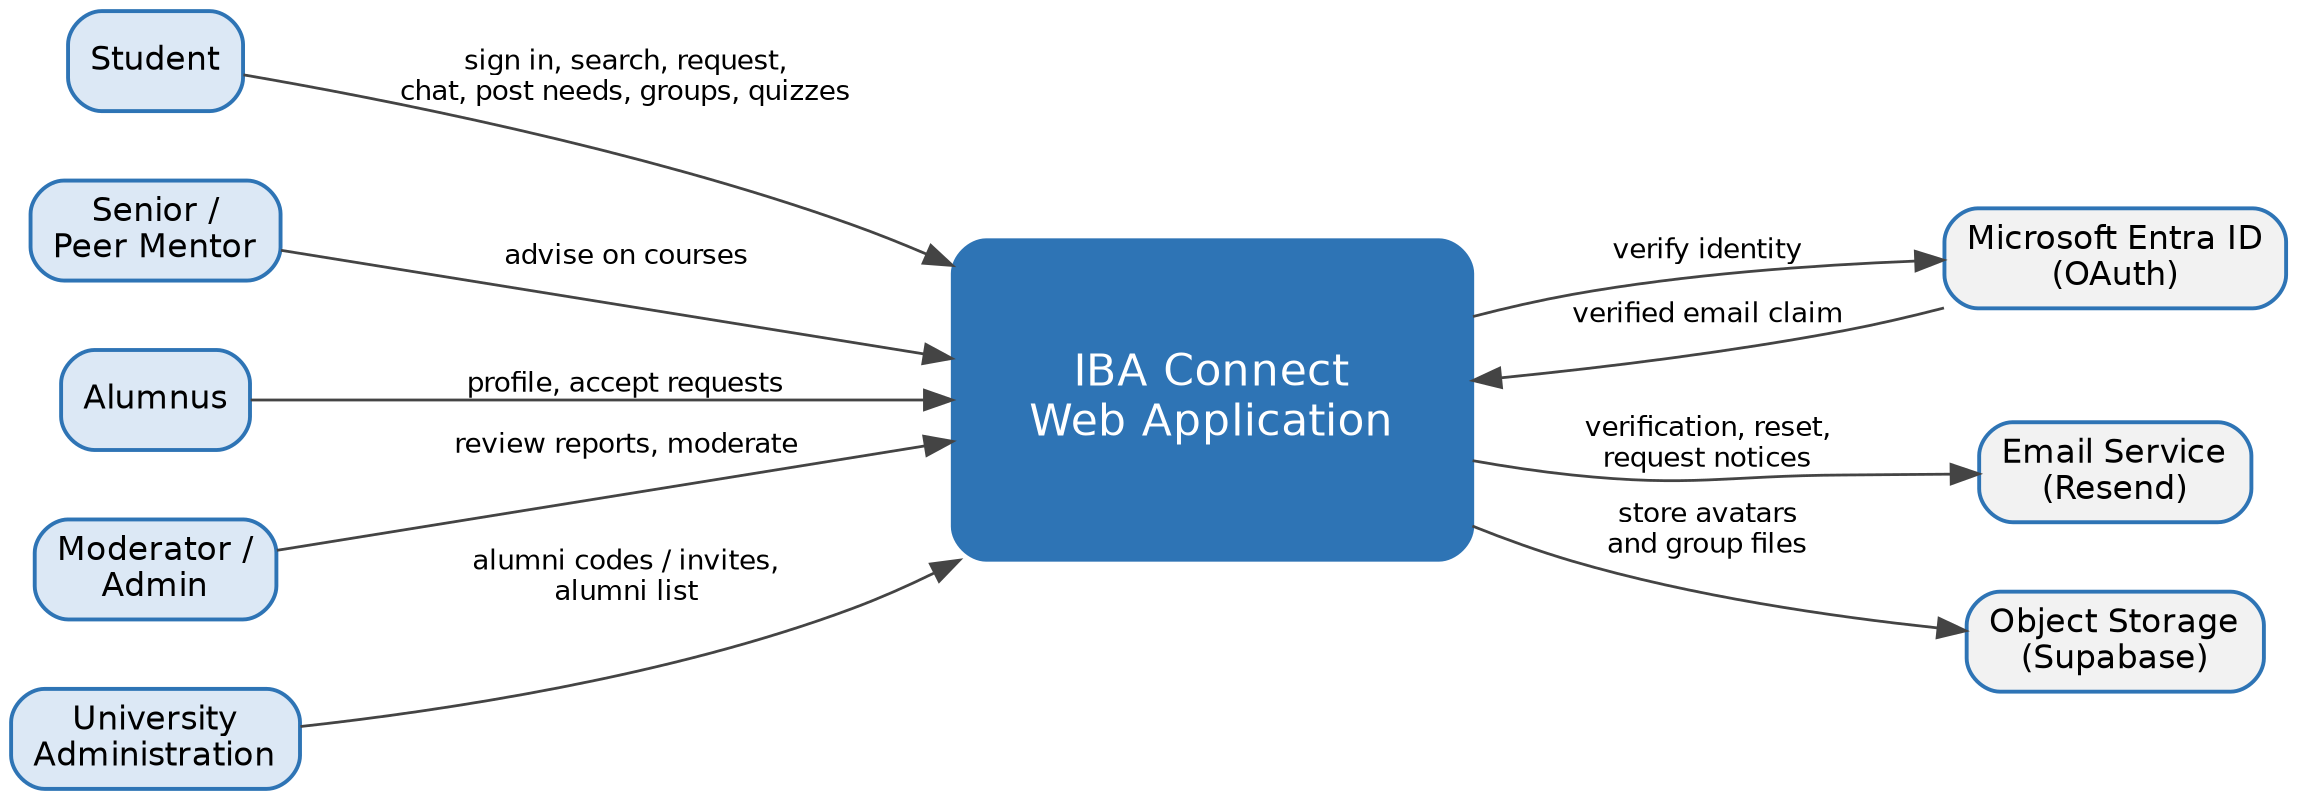
\includegraphics[width=0.95\linewidth,height=0.8\textheight,keepaspectratio]{figures/fig01.png}
\caption{Context diagram of IBA Connect}\end{figure}
\subsection{Use Case Diagrams}
Verified User is an abstract actor. Student, Alumnus and Senior inherit from it, and Senior also inherits from Student.

\begin{figure}[H]\centering
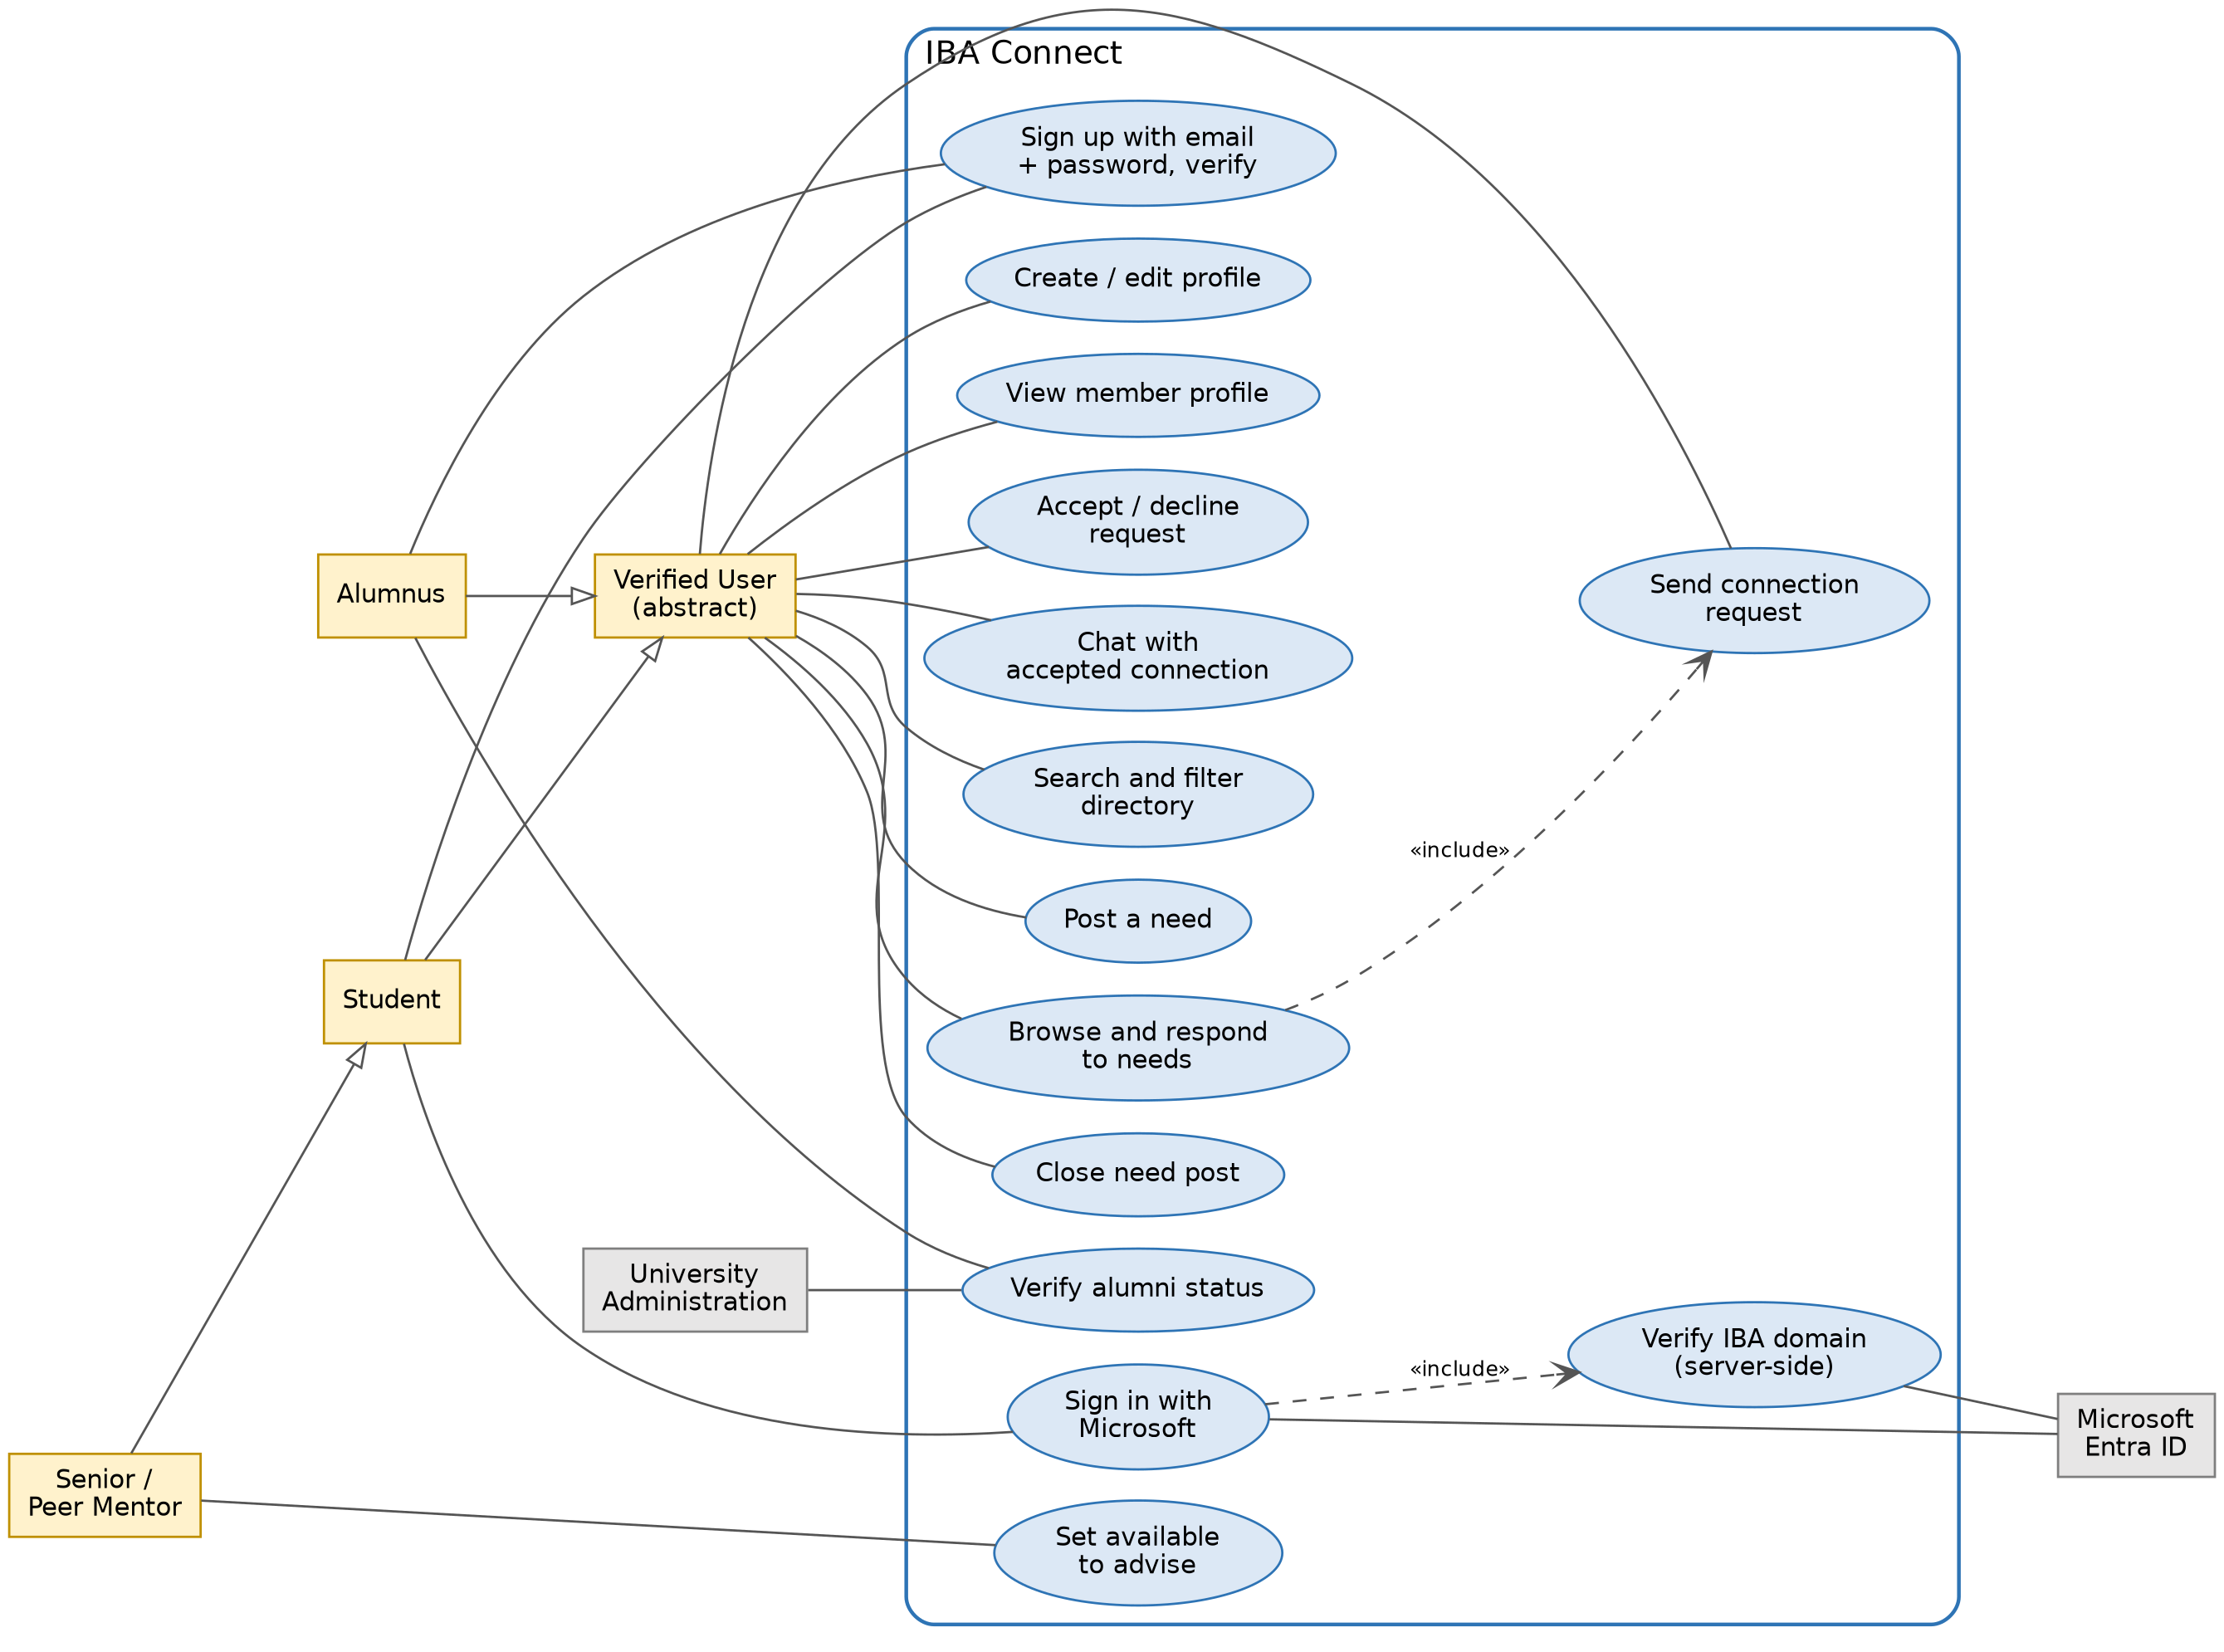
\includegraphics[width=0.95\linewidth,height=0.8\textheight,keepaspectratio]{figures/fig02.png}
\caption{Use cases: identity, discovery, connections and need board}\end{figure}
\begin{figure}[H]\centering
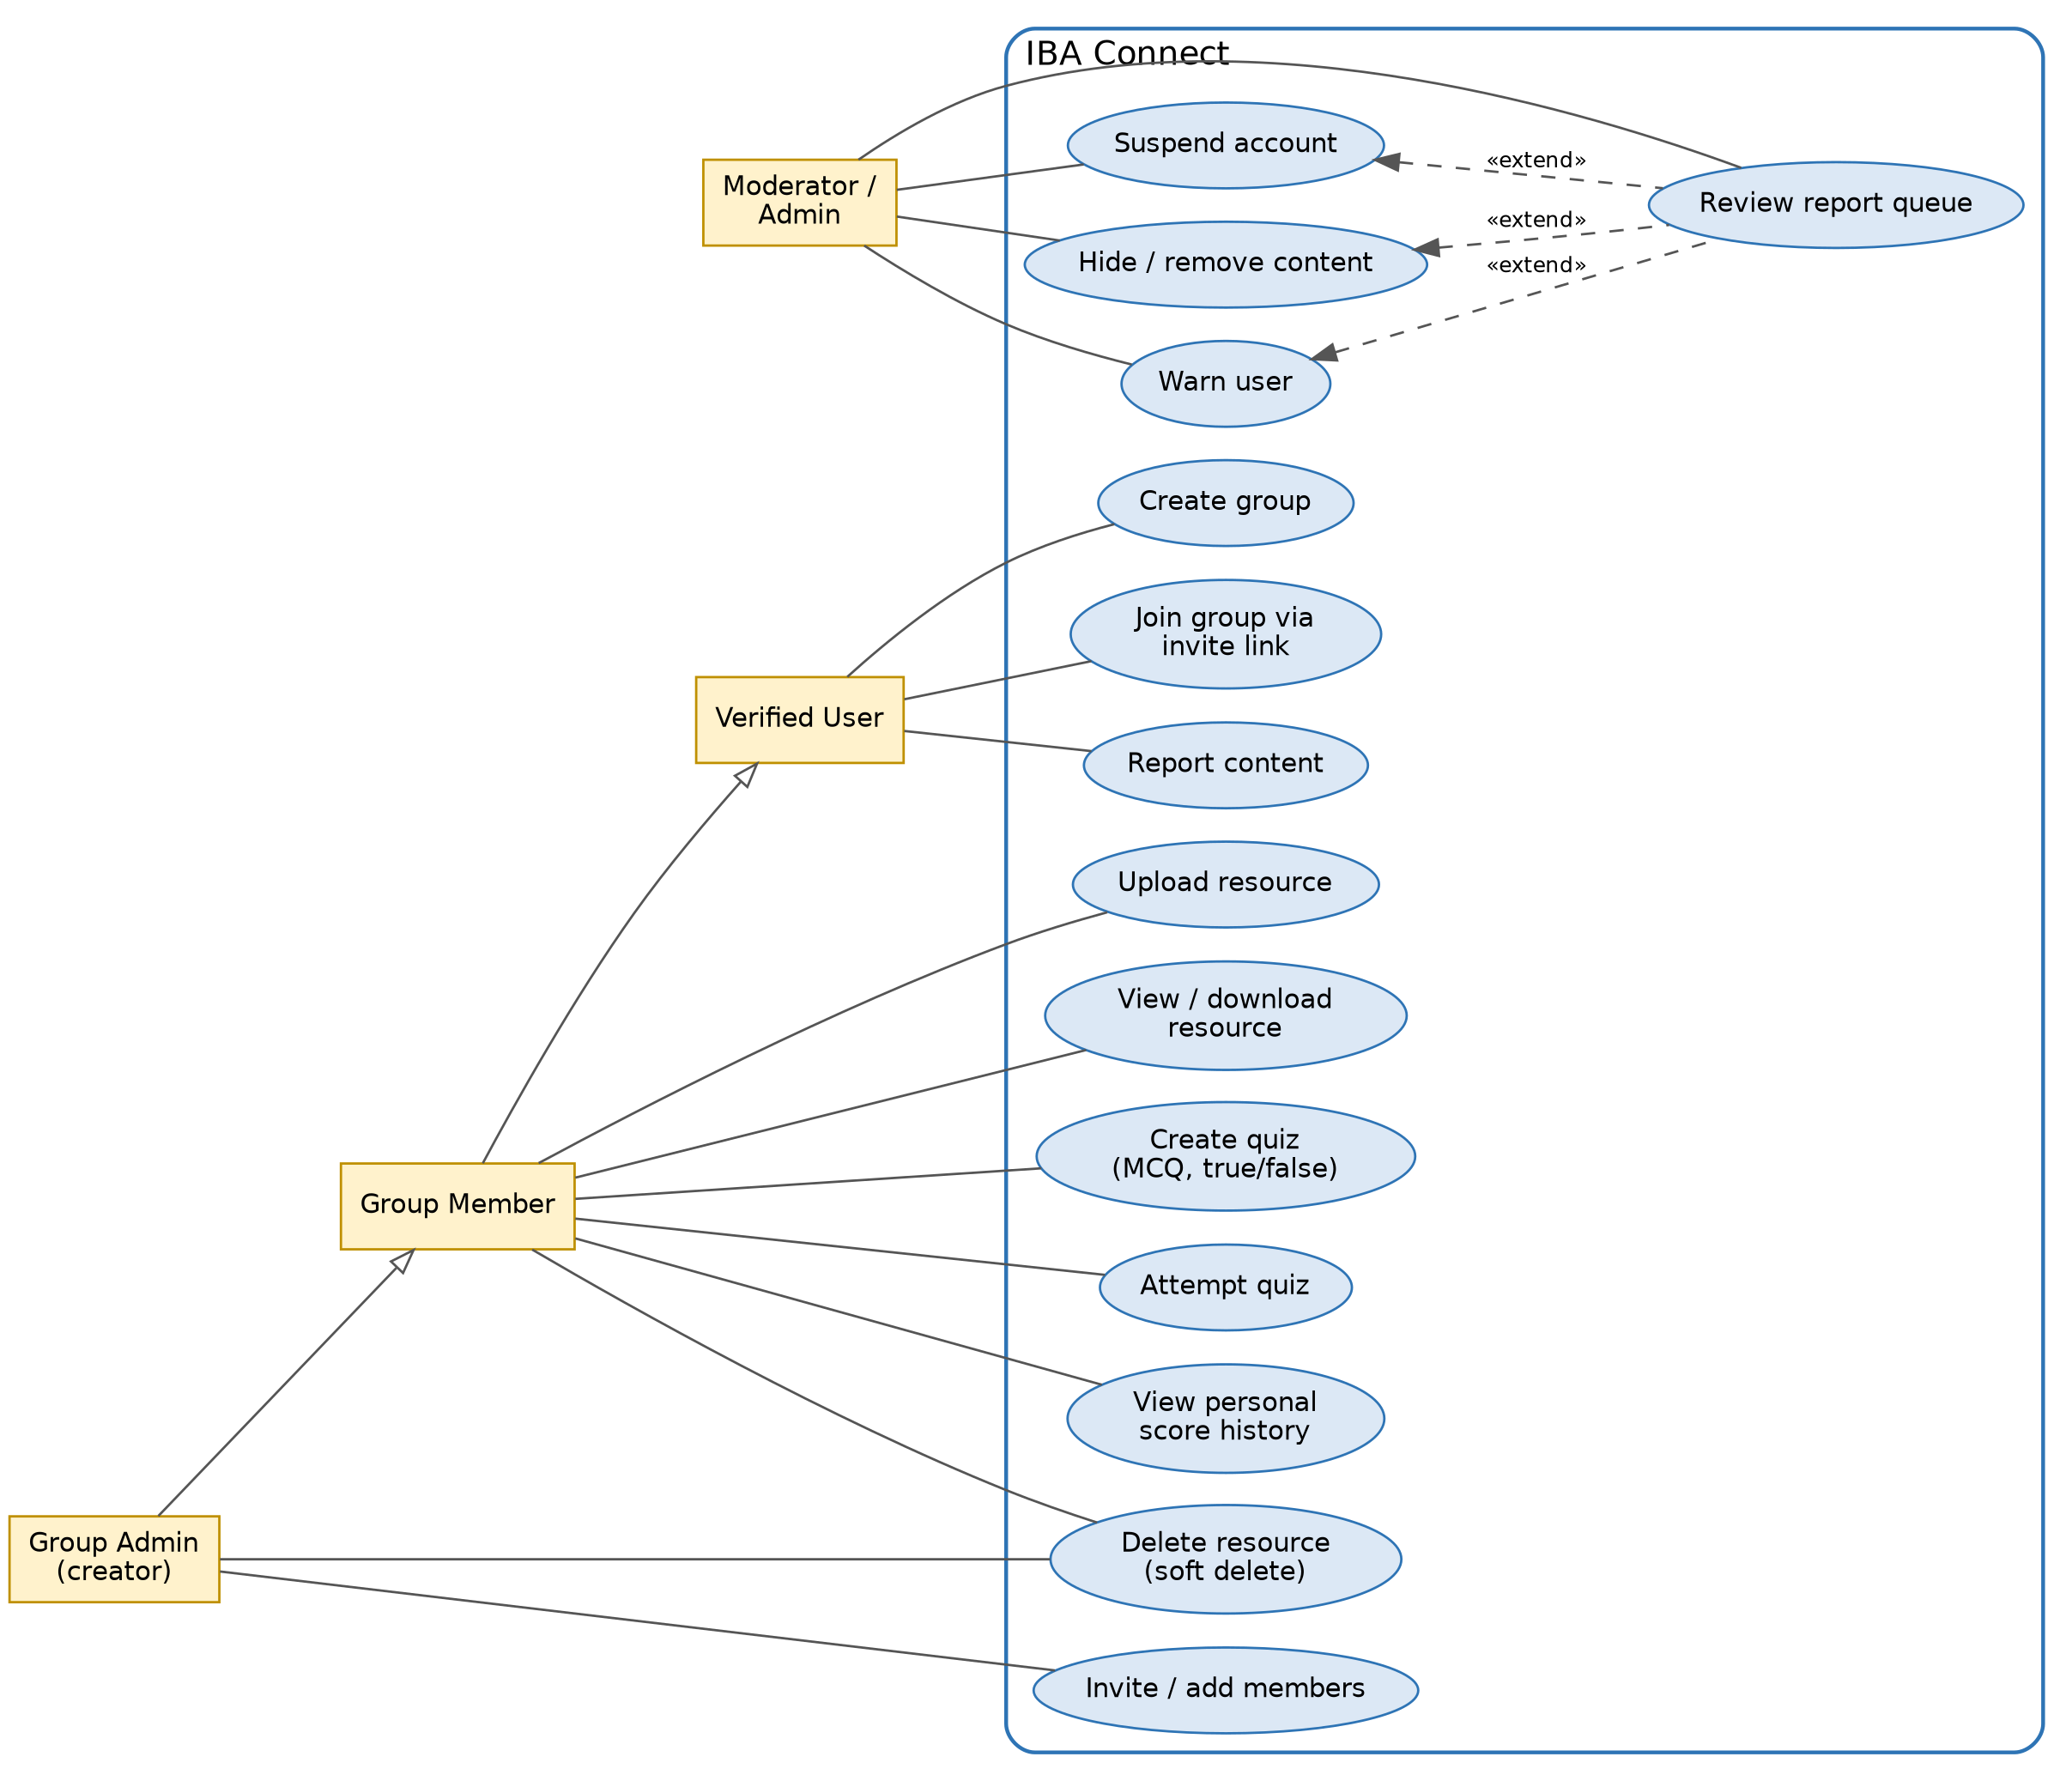
\includegraphics[width=0.95\linewidth,height=0.8\textheight,keepaspectratio]{figures/fig03.png}
\caption{Use cases: groups, resources, quizzes and moderation}\end{figure}
\subsection{Architecture Diagram}
IBA Connect uses a layered architecture on Next.js with a versioned REST API, PostgreSQL through Prisma, and three external services.

\begin{figure}[H]\centering
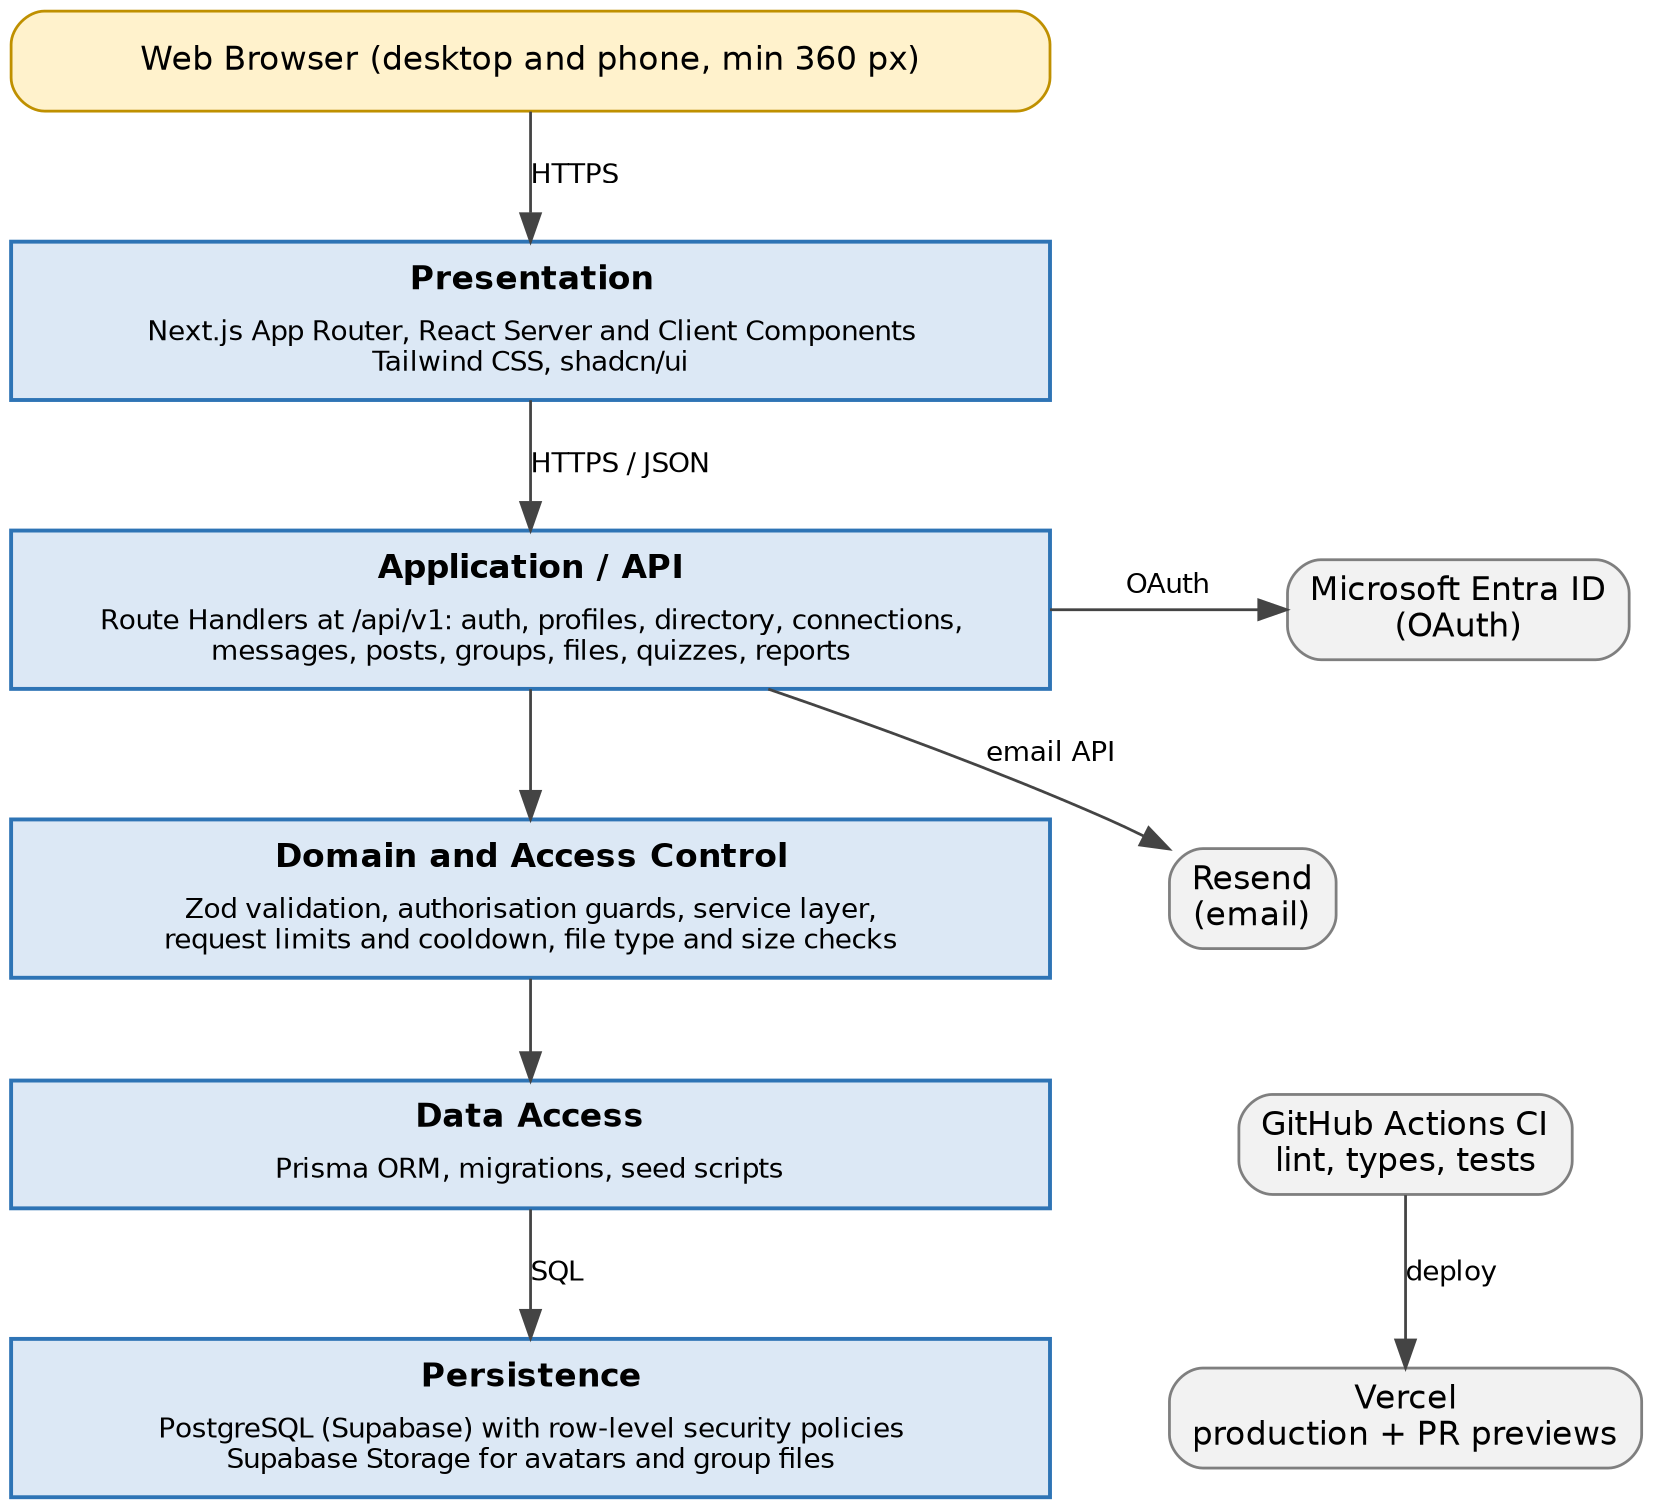
\includegraphics[width=0.7\linewidth,height=0.8\textheight,keepaspectratio]{figures/fig04.png}
\caption{Layered architecture and deployment topology (Email: Brevo from v1.1.)}\end{figure}
\subsection{Entity Relationship Diagrams}
The data model is shown in five parts. PK is a primary key and FK a foreign key. A line with a crow's foot is one-to-many, a line with a bar at both ends is one-to-one, and a dashed line is an optional or secondary relationship. Entities repeated from another figure are shown in short form.

\begin{figure}[H]\centering
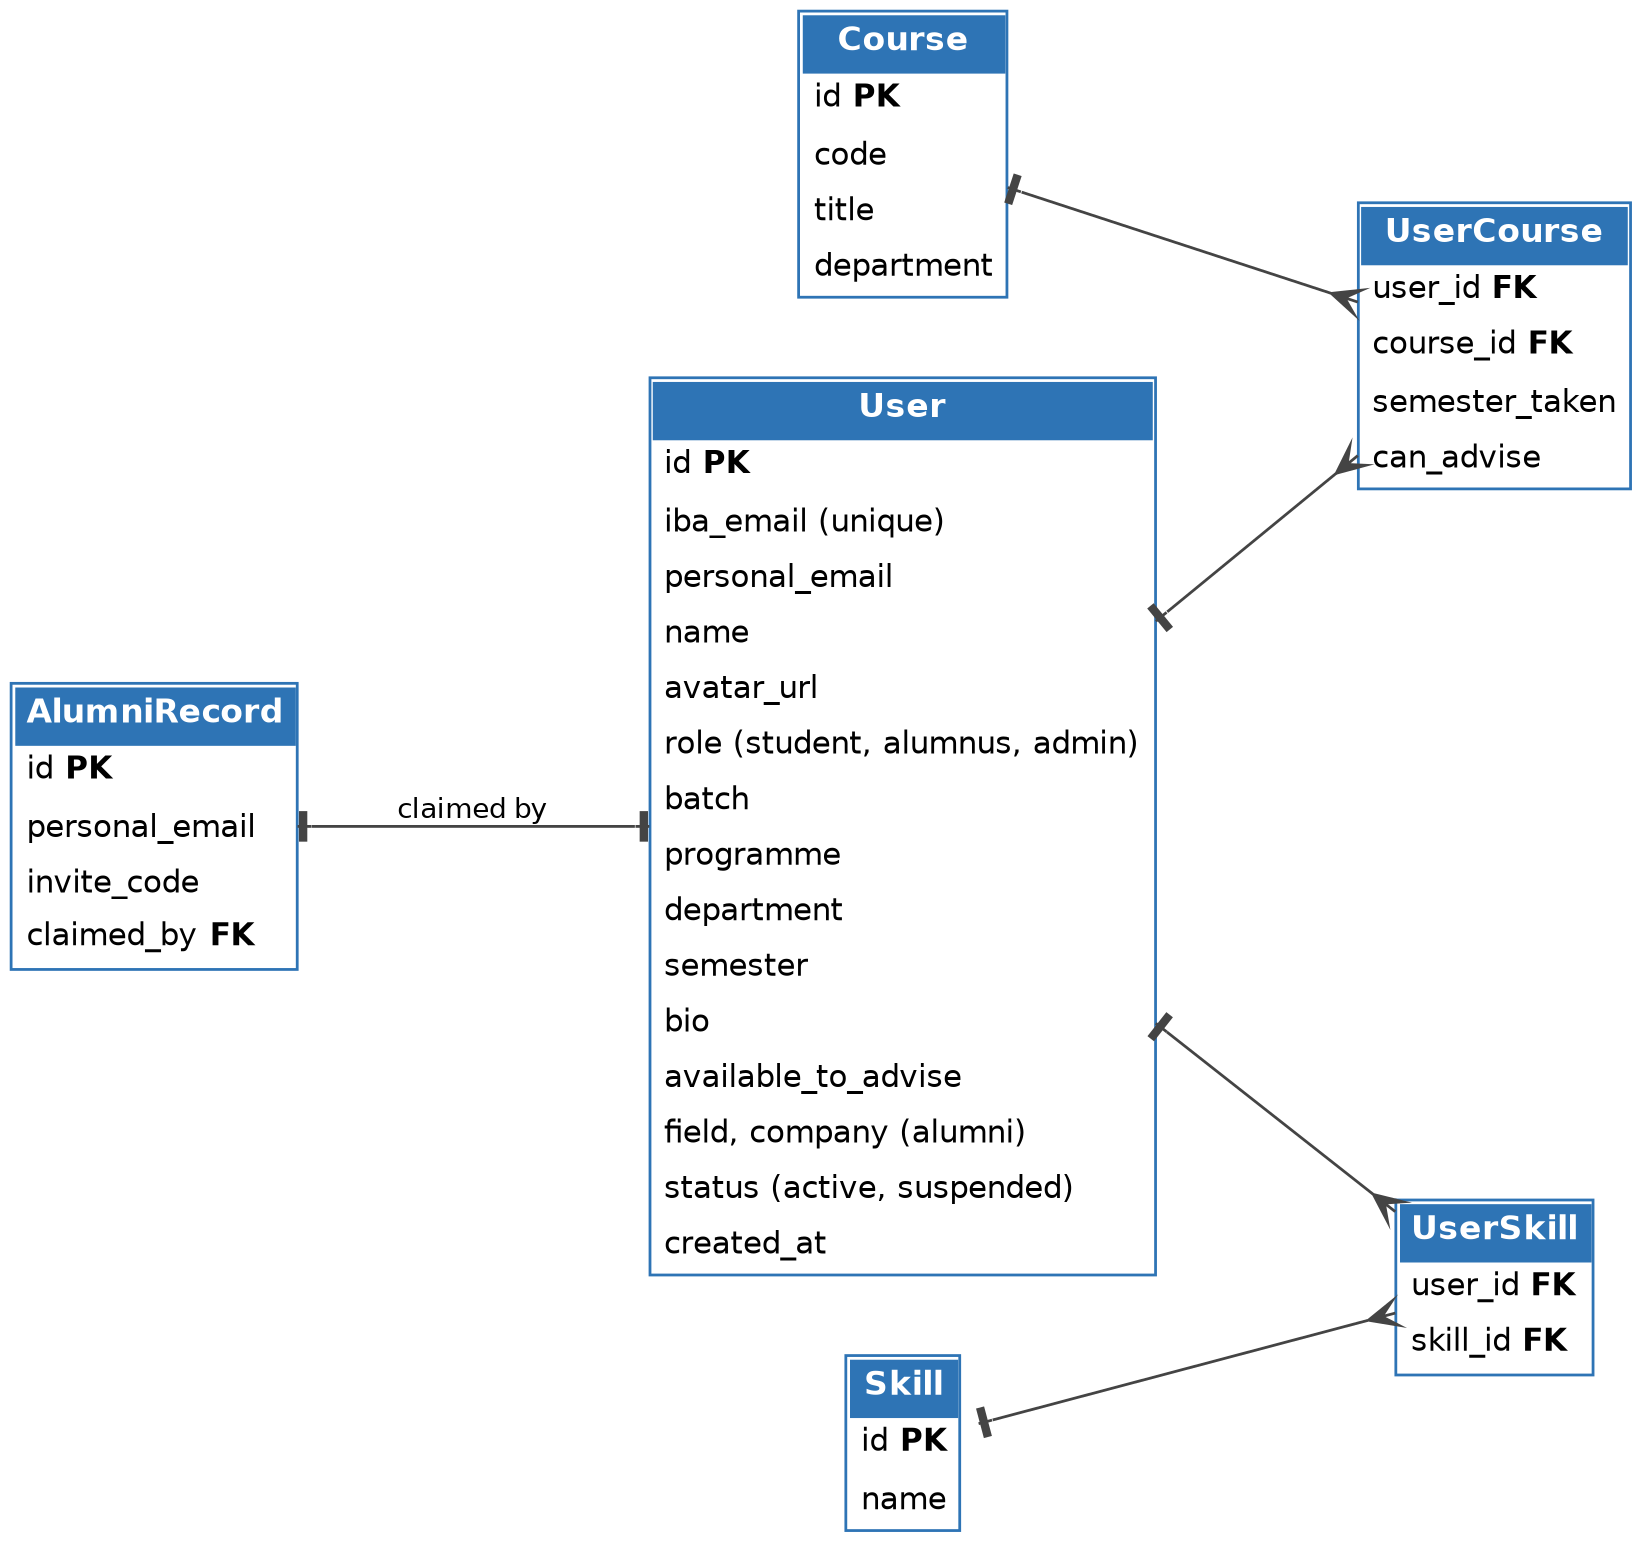
\includegraphics[width=0.95\linewidth,height=0.8\textheight,keepaspectratio]{figures/fig05.png}
\caption{ERD part 1: users, profiles, courses, skills and alumni verification}\end{figure}
\begin{figure}[H]\centering
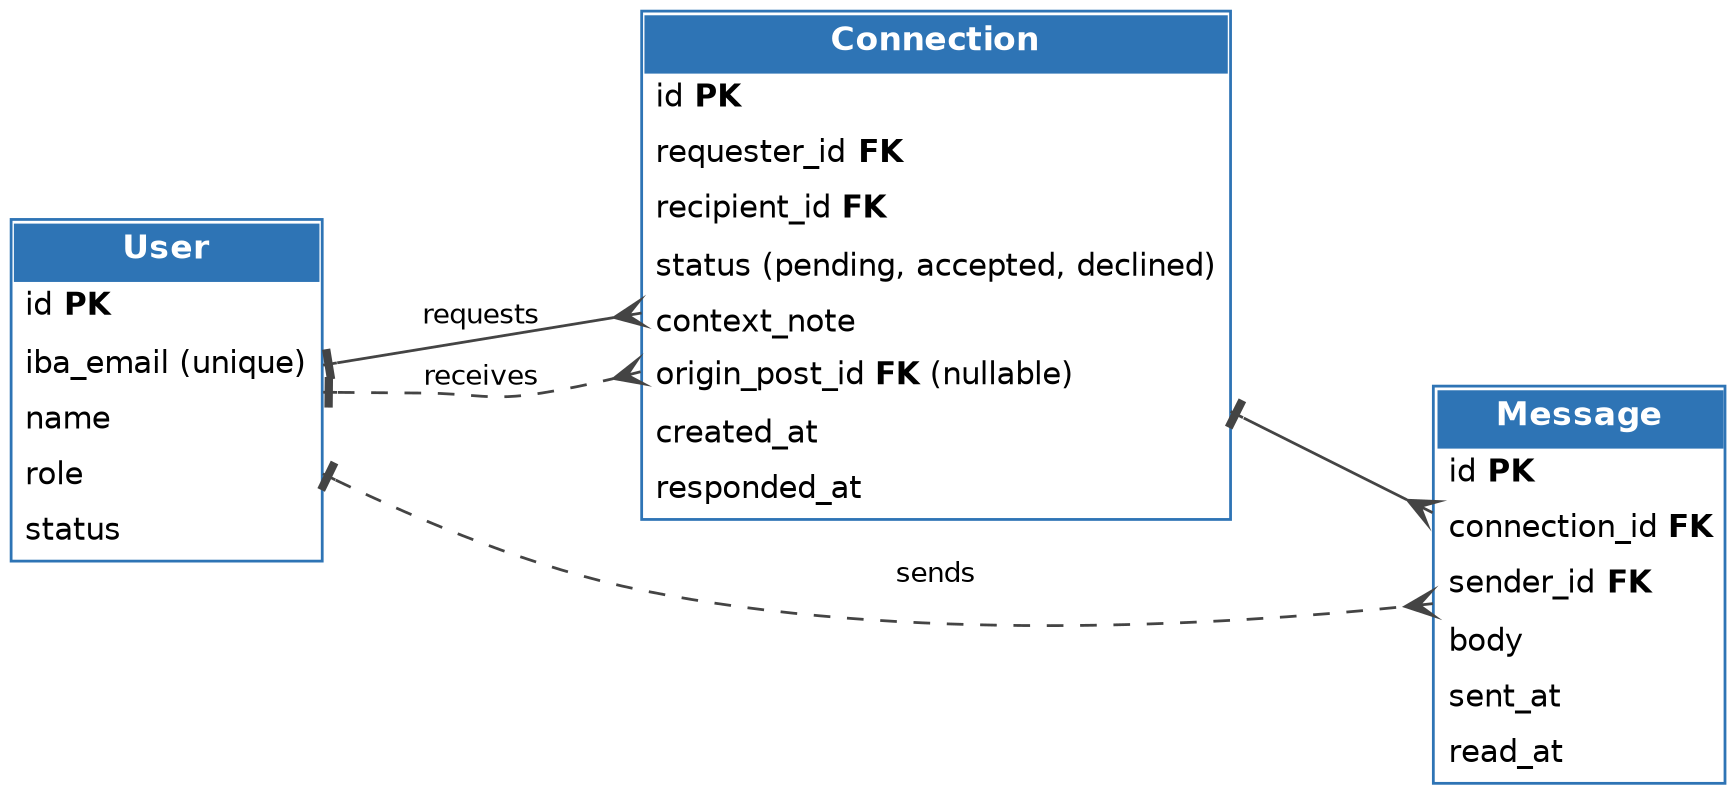
\includegraphics[width=0.95\linewidth,height=0.8\textheight,keepaspectratio]{figures/fig06.png}
\caption{ERD part 2: connections and messages}\end{figure}
\begin{figure}[H]\centering
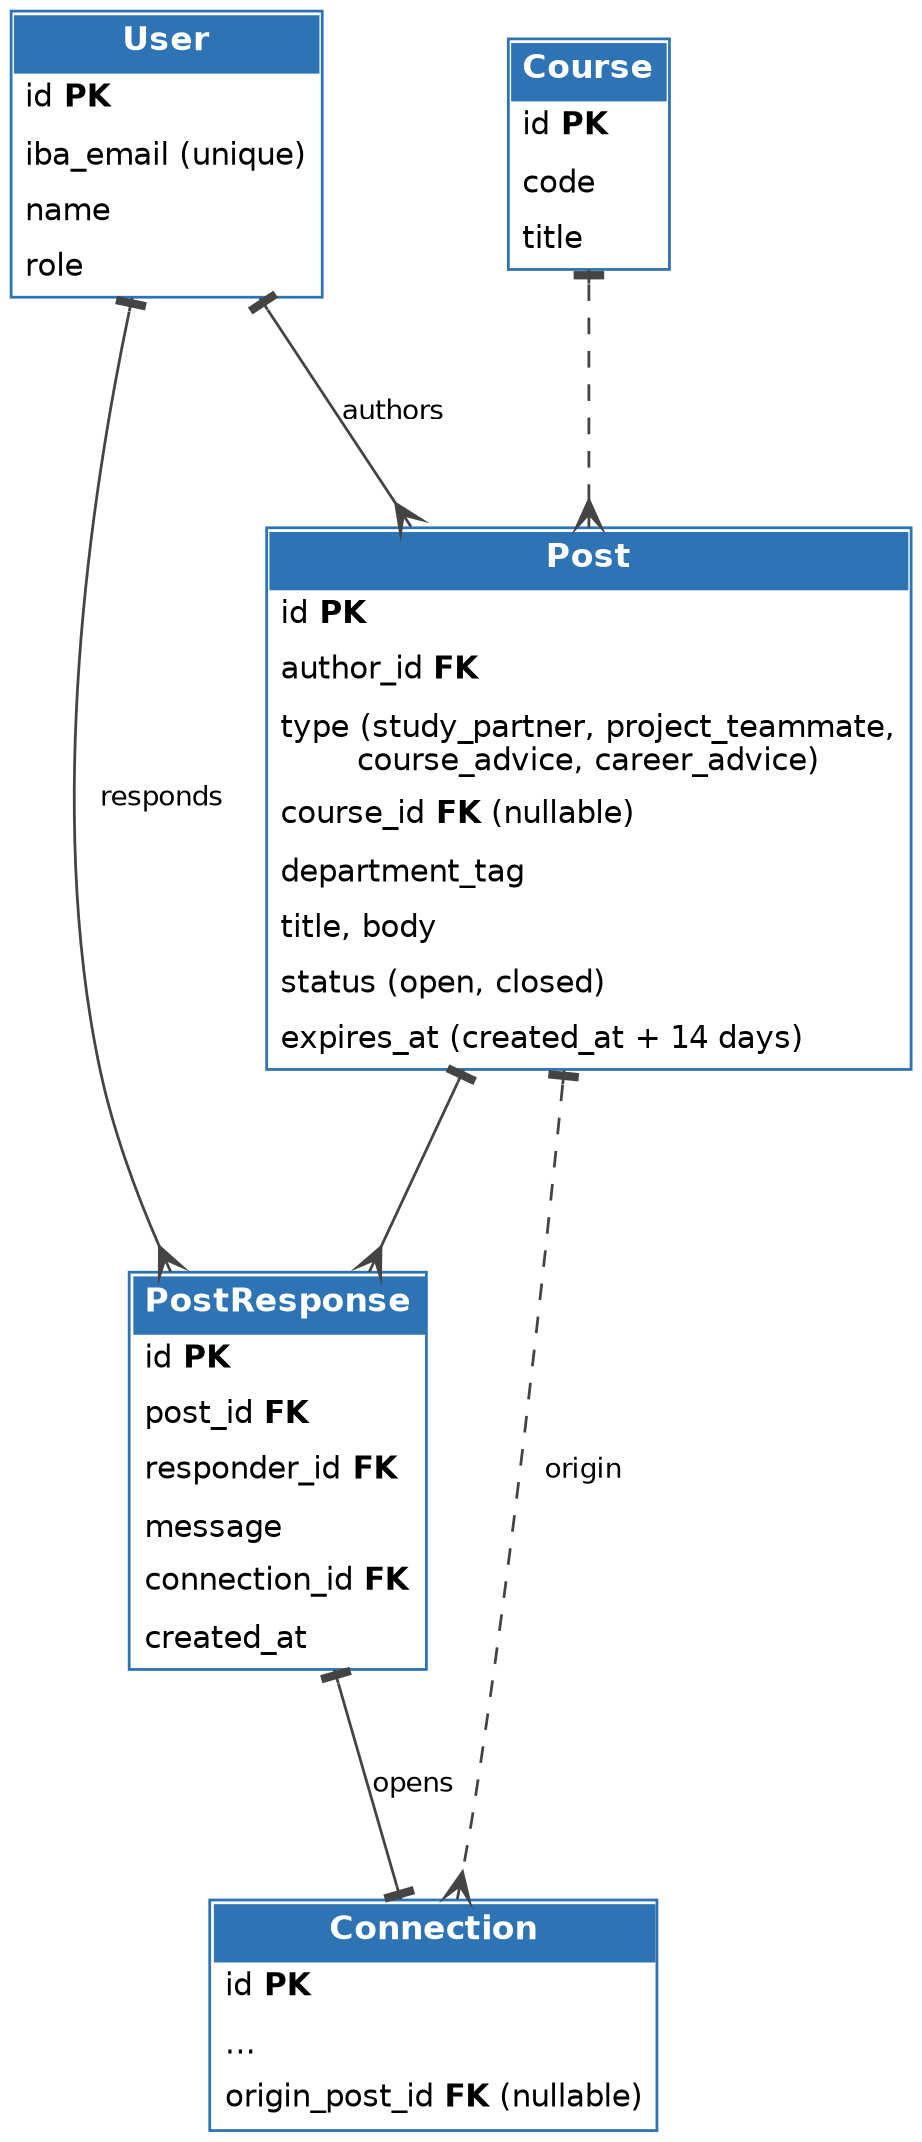
\includegraphics[width=0.95\linewidth,height=0.8\textheight,keepaspectratio]{figures/fig07.png}
\caption{ERD part 3: need board posts and responses}\end{figure}
\begin{figure}[H]\centering
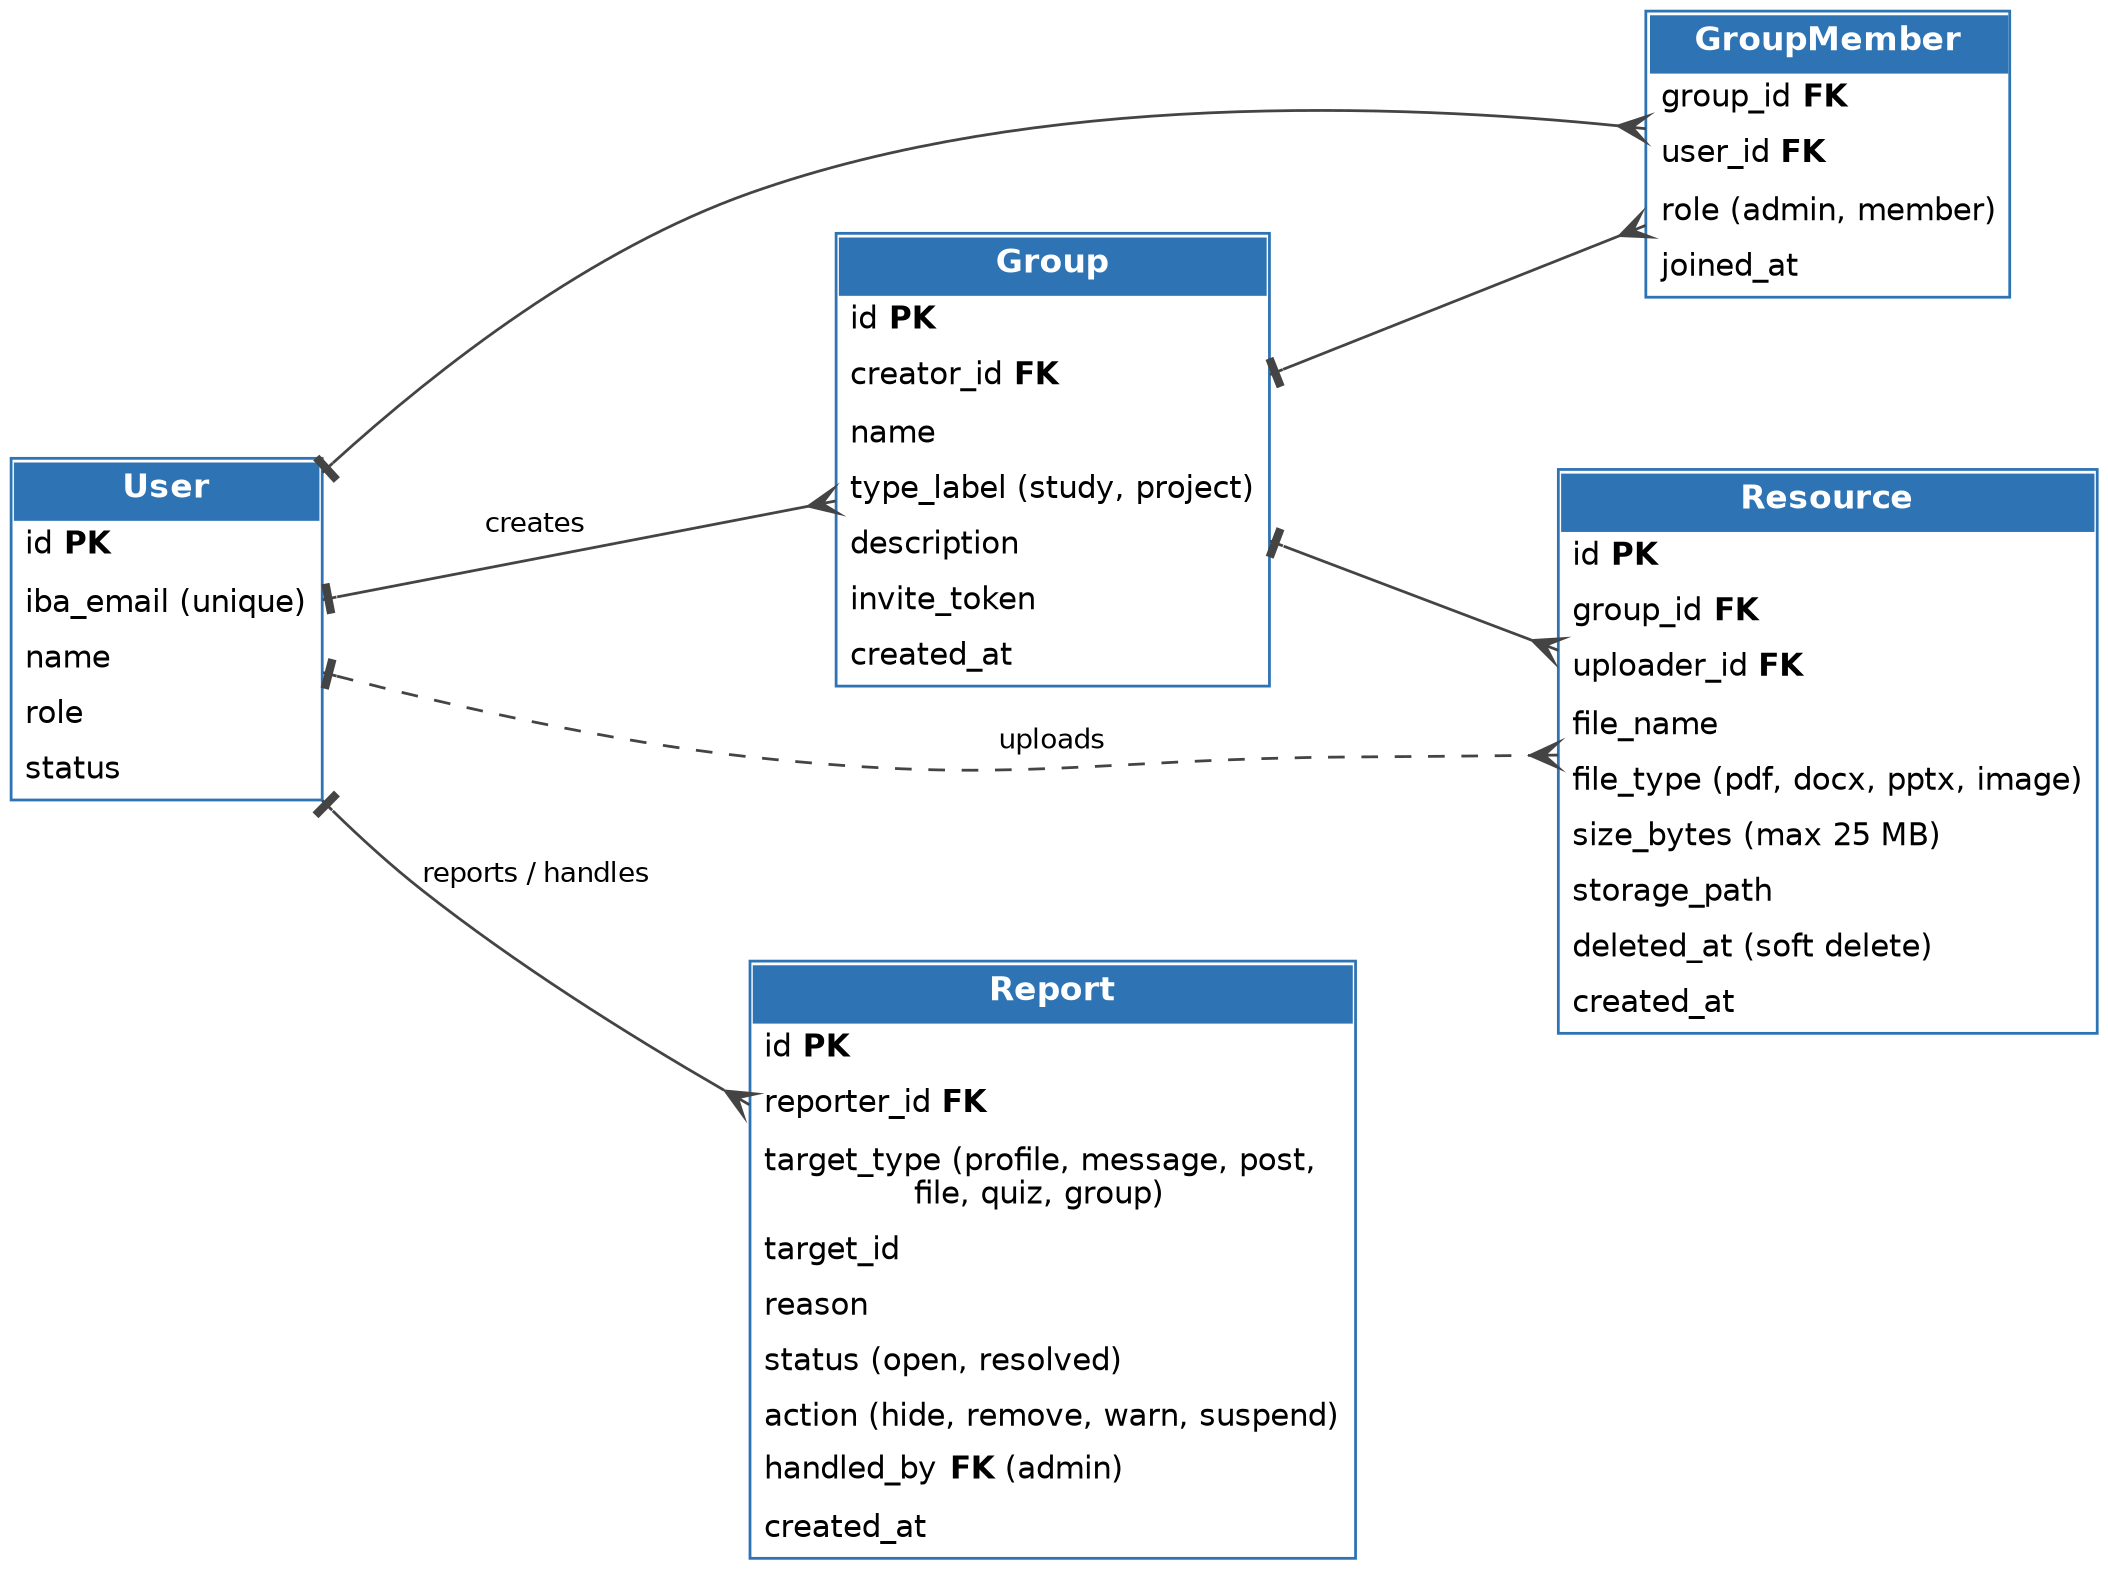
\includegraphics[width=0.95\linewidth,height=0.8\textheight,keepaspectratio]{figures/fig08.png}
\caption{ERD part 4: groups, resources and reports}\end{figure}
\begin{figure}[H]\centering
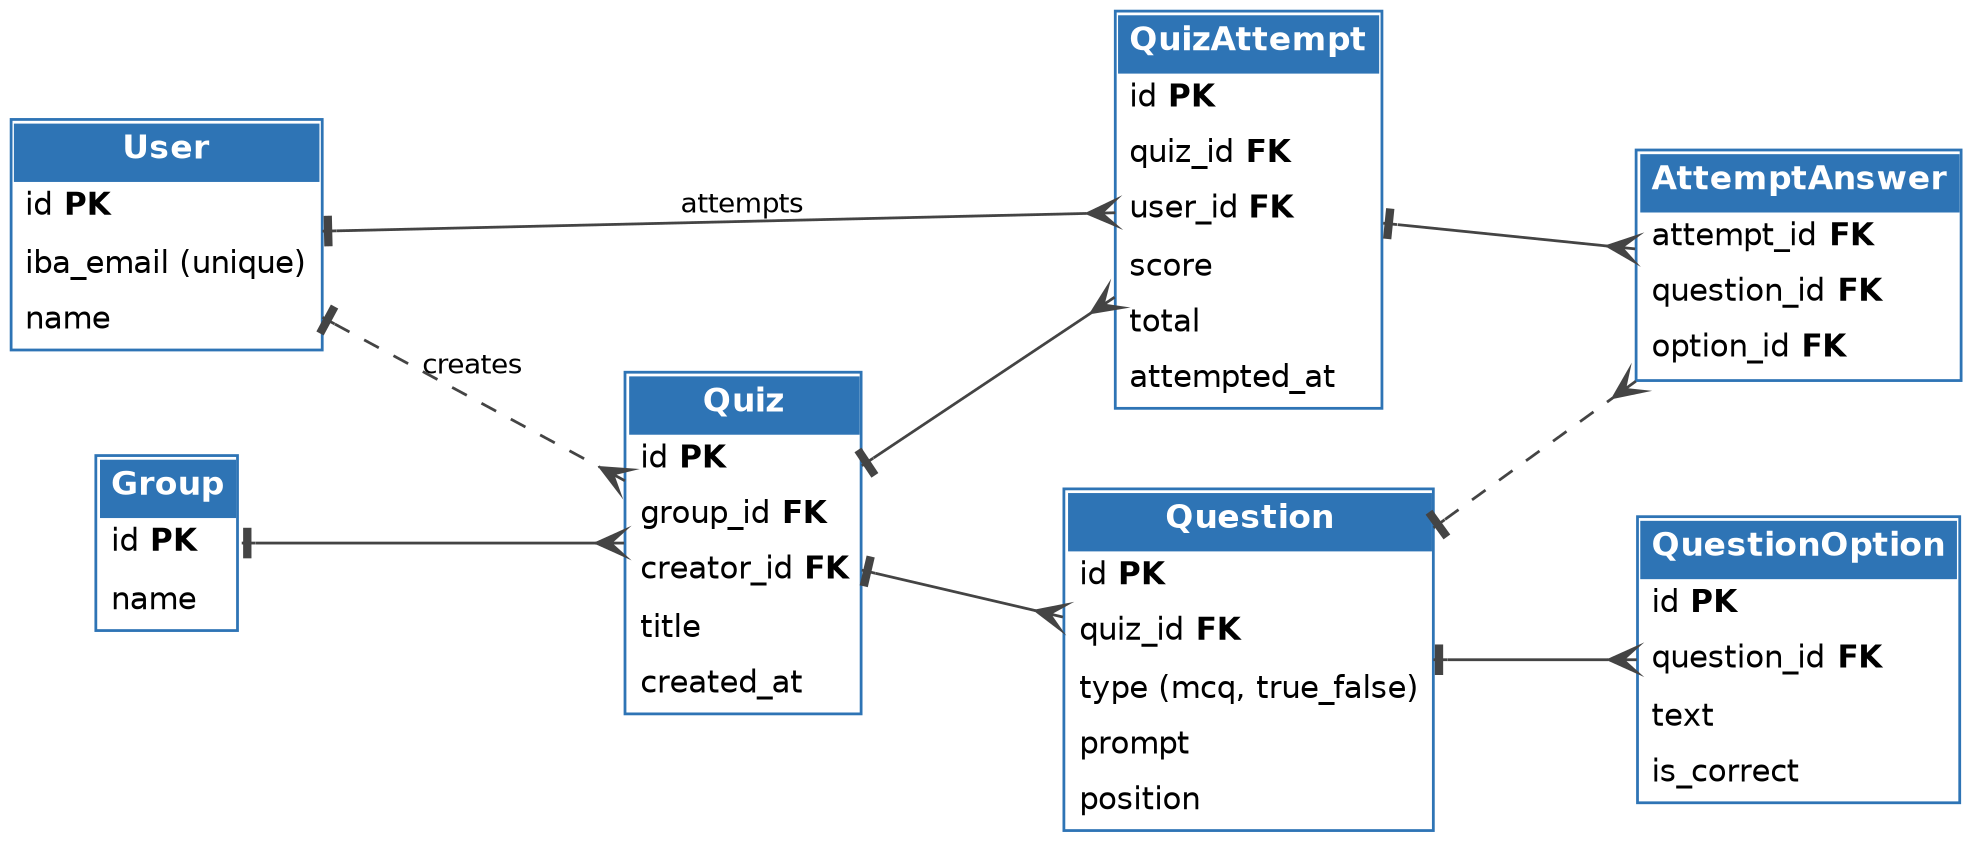
\includegraphics[width=0.95\linewidth,height=0.8\textheight,keepaspectratio]{figures/fig09.png}
\caption{ERD part 5: quizzes, attempts and scores}\end{figure}
\subsection{Sequence Diagrams}
The three sequence diagrams show the most important flows: Microsoft sign-in with domain enforcement, a connection request through to chat, and group file upload and download.

\begin{figure}[H]\centering
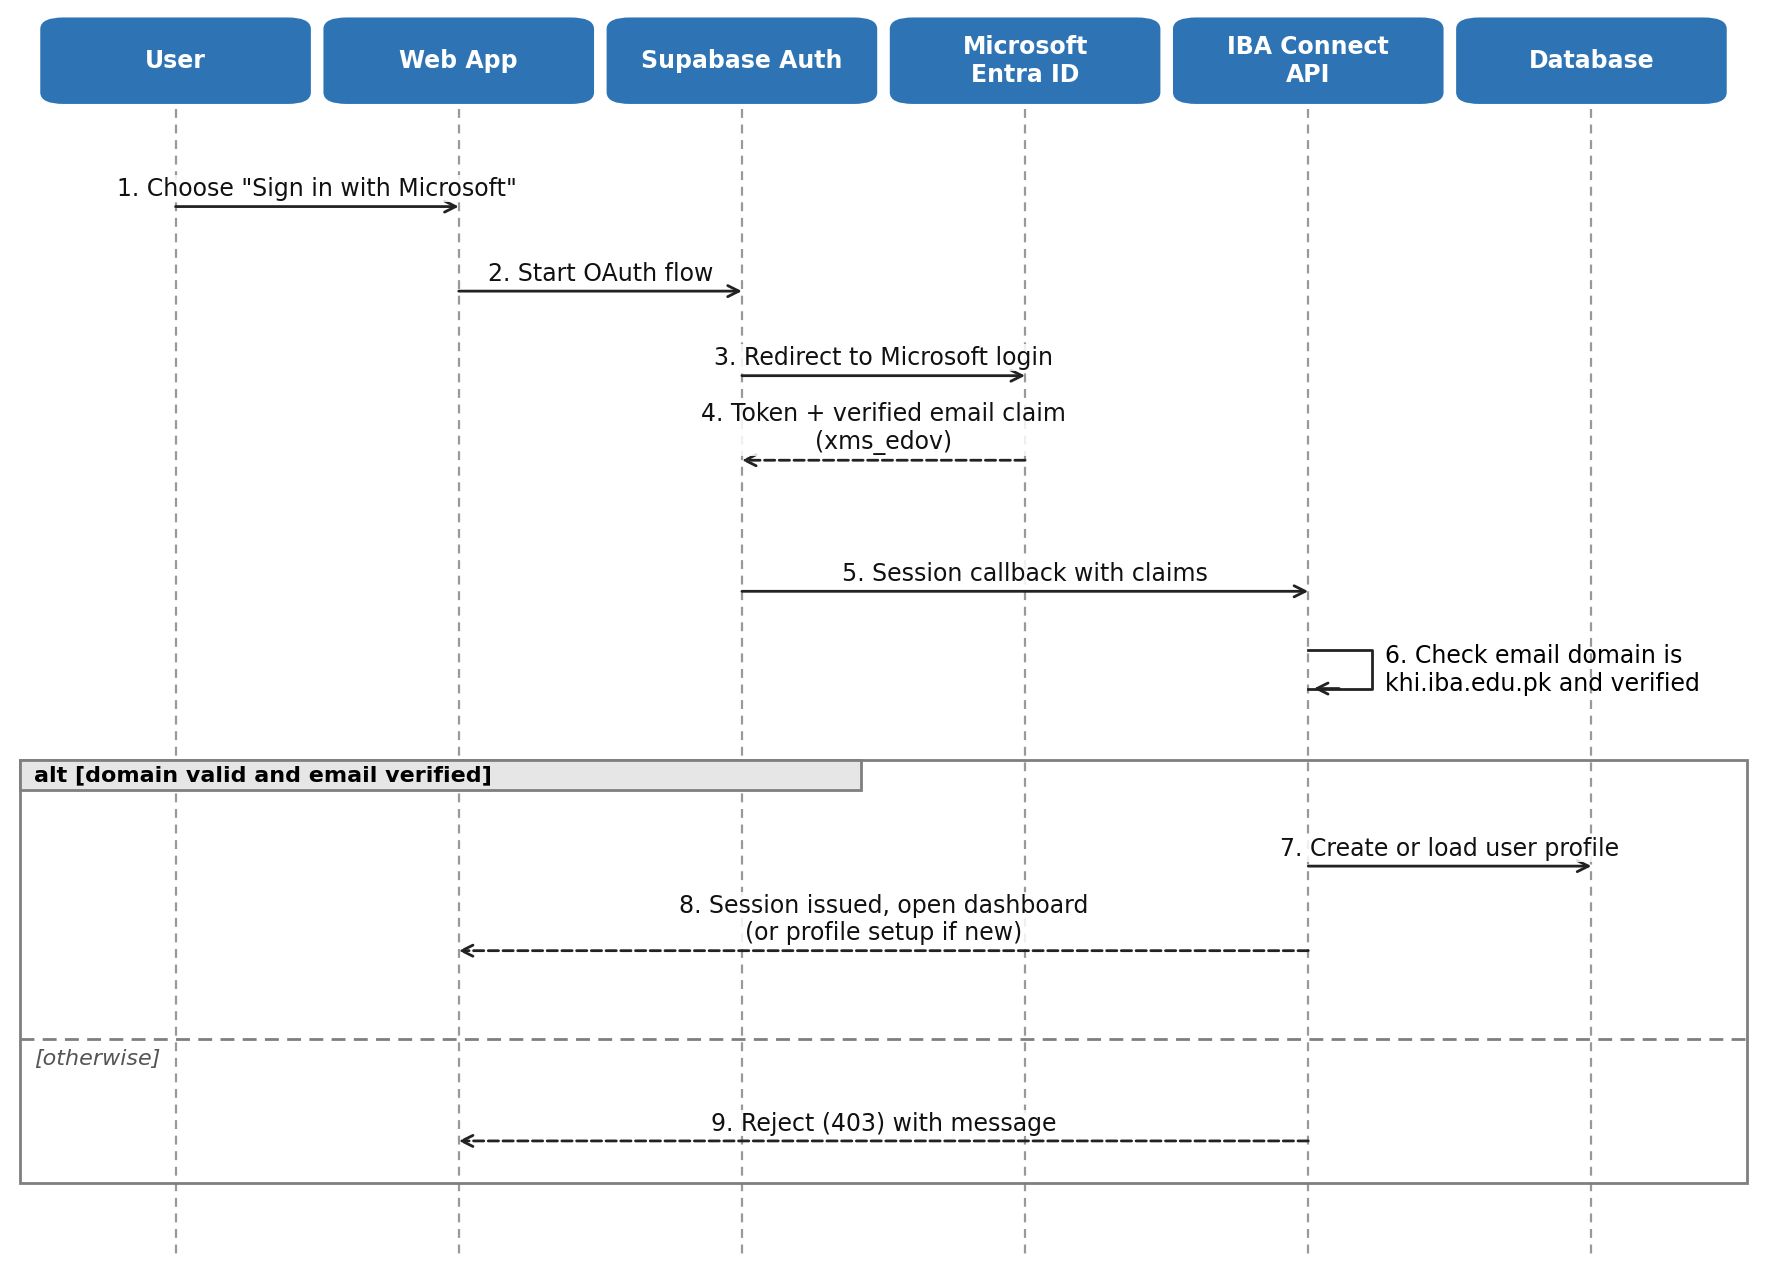
\includegraphics[width=0.95\linewidth,height=0.8\textheight,keepaspectratio]{figures/fig10.png}
\caption{Sequence: sign in with Microsoft and domain verification}\end{figure}
\begin{figure}[H]\centering
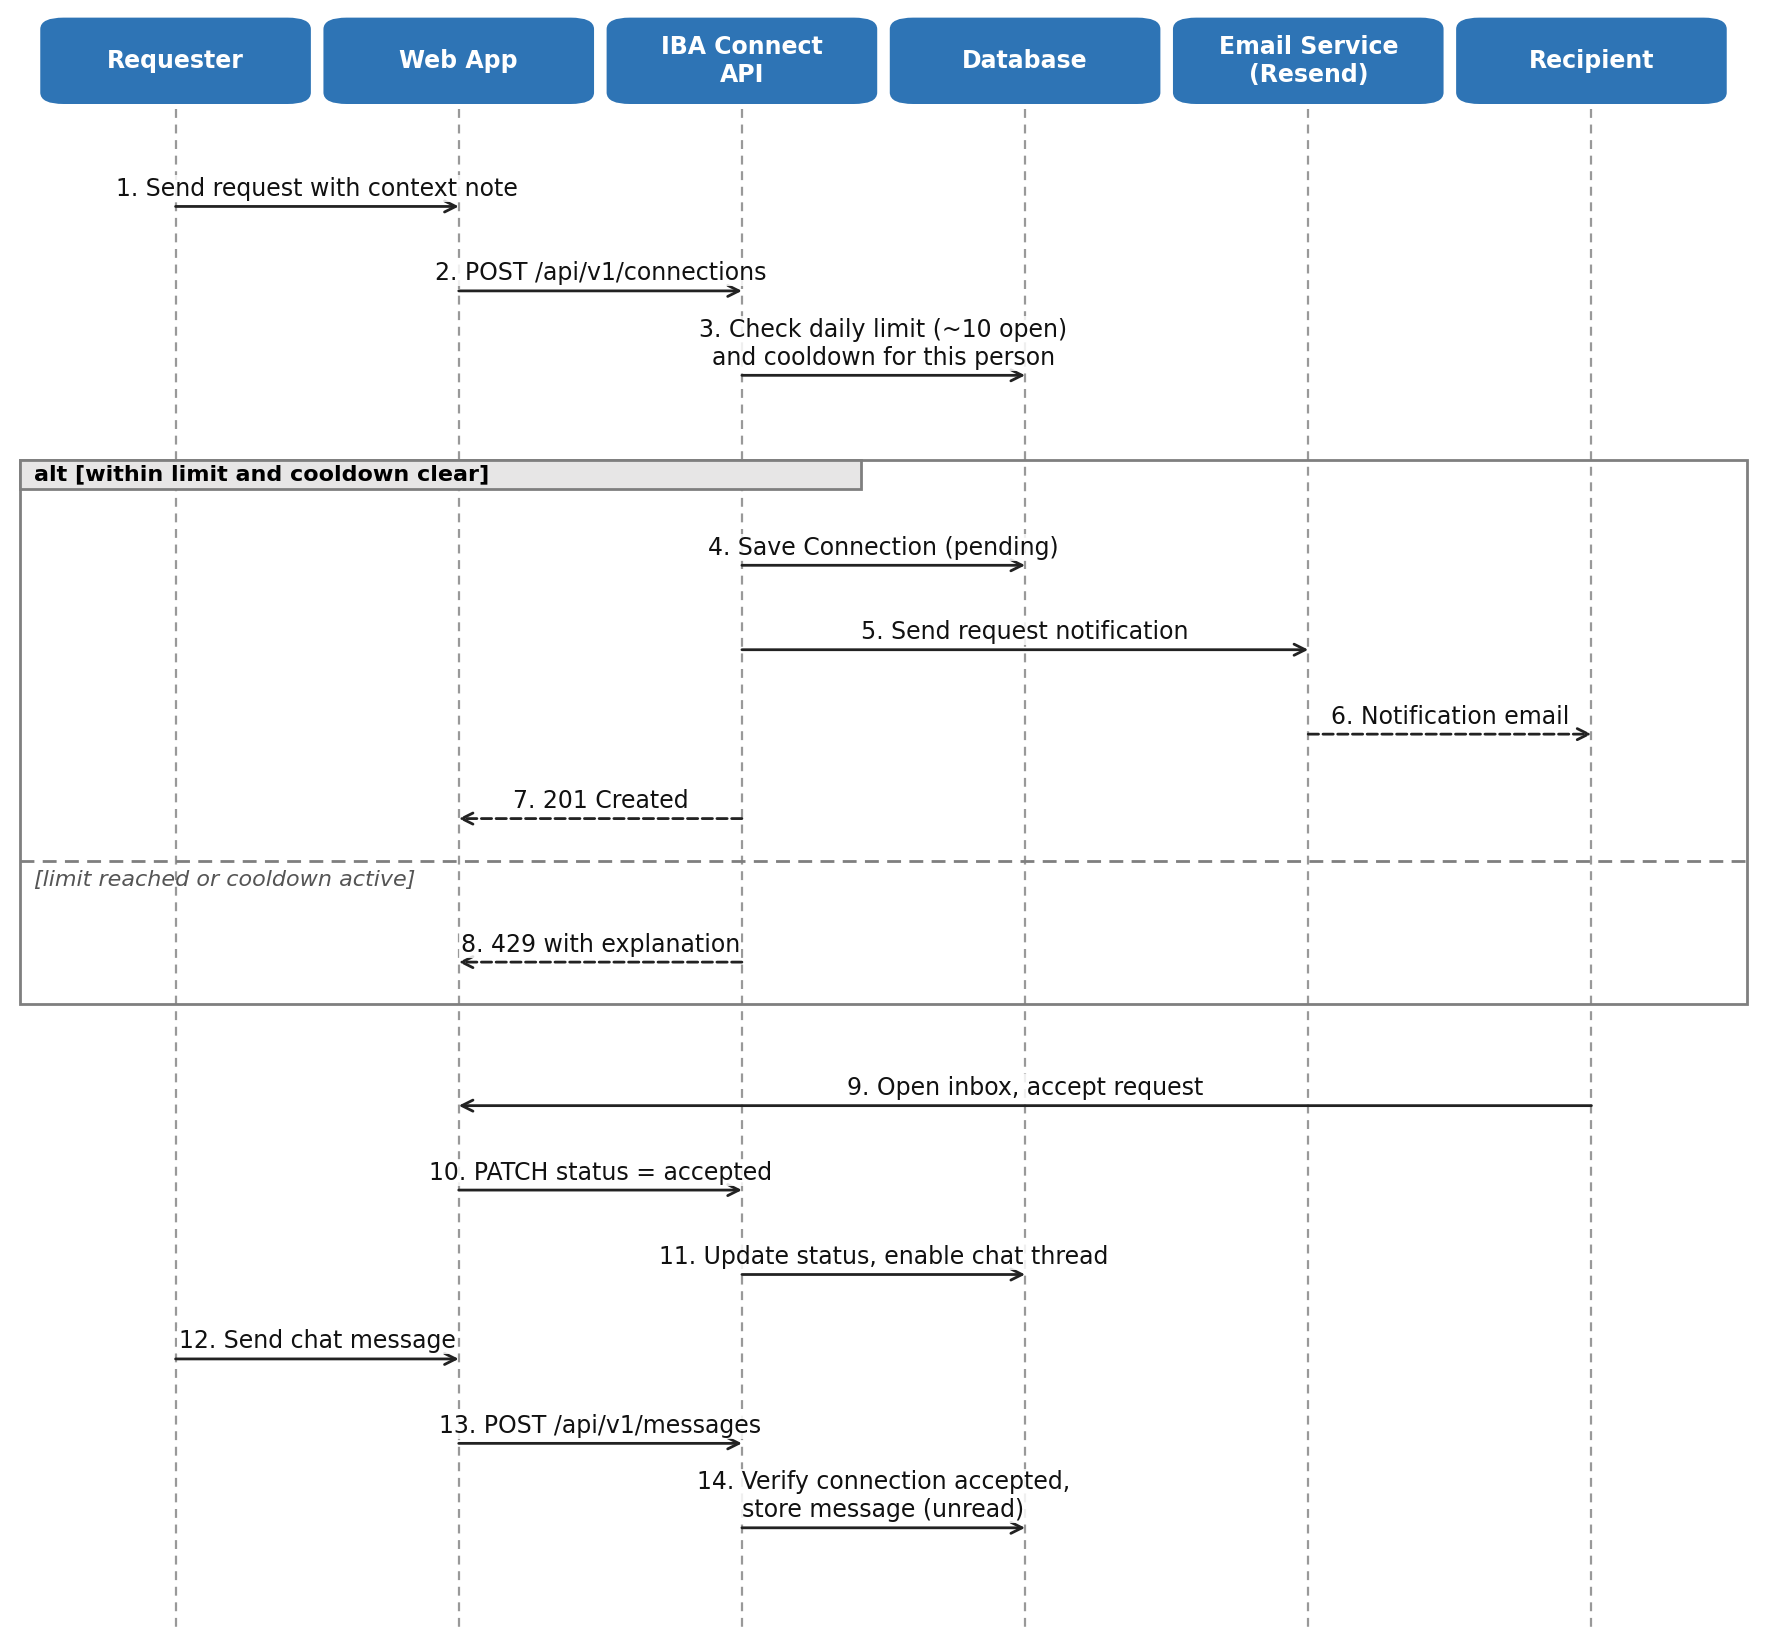
\includegraphics[width=0.95\linewidth,height=0.8\textheight,keepaspectratio]{figures/fig11.png}
\caption{Sequence: connection request, acceptance and chat}\end{figure}
\begin{figure}[H]\centering
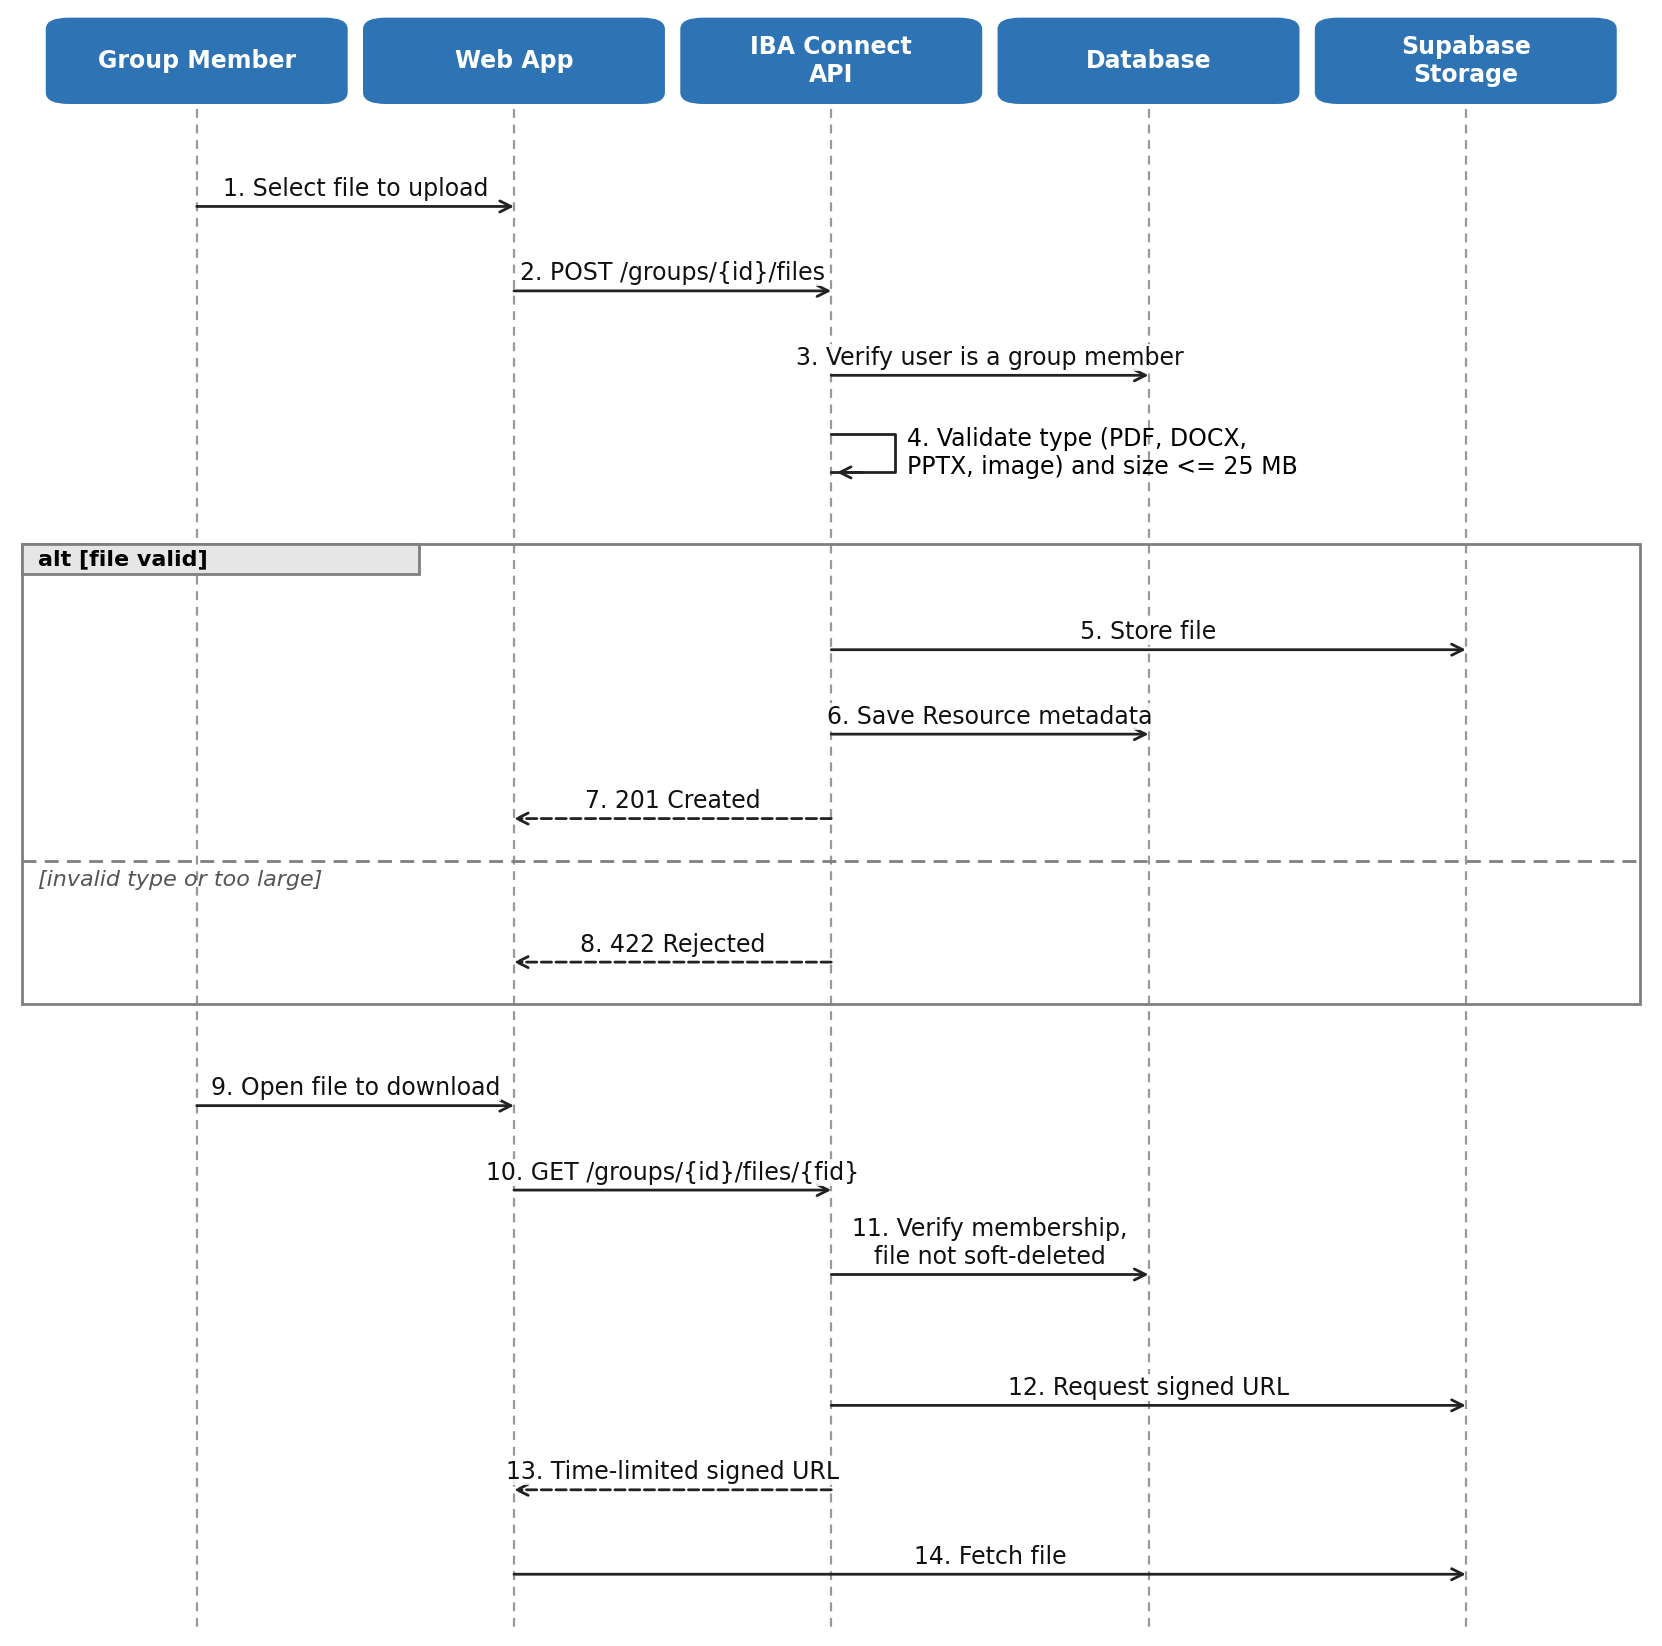
\includegraphics[width=0.95\linewidth,height=0.8\textheight,keepaspectratio]{figures/fig12.png}
\caption{Sequence: group resource upload and download}\end{figure}
\subsection{State Diagrams}
The state diagrams show the life cycle of the four objects whose status changes: connection requests, need-board posts, group files, and user accounts.

\begin{figure}[H]\centering
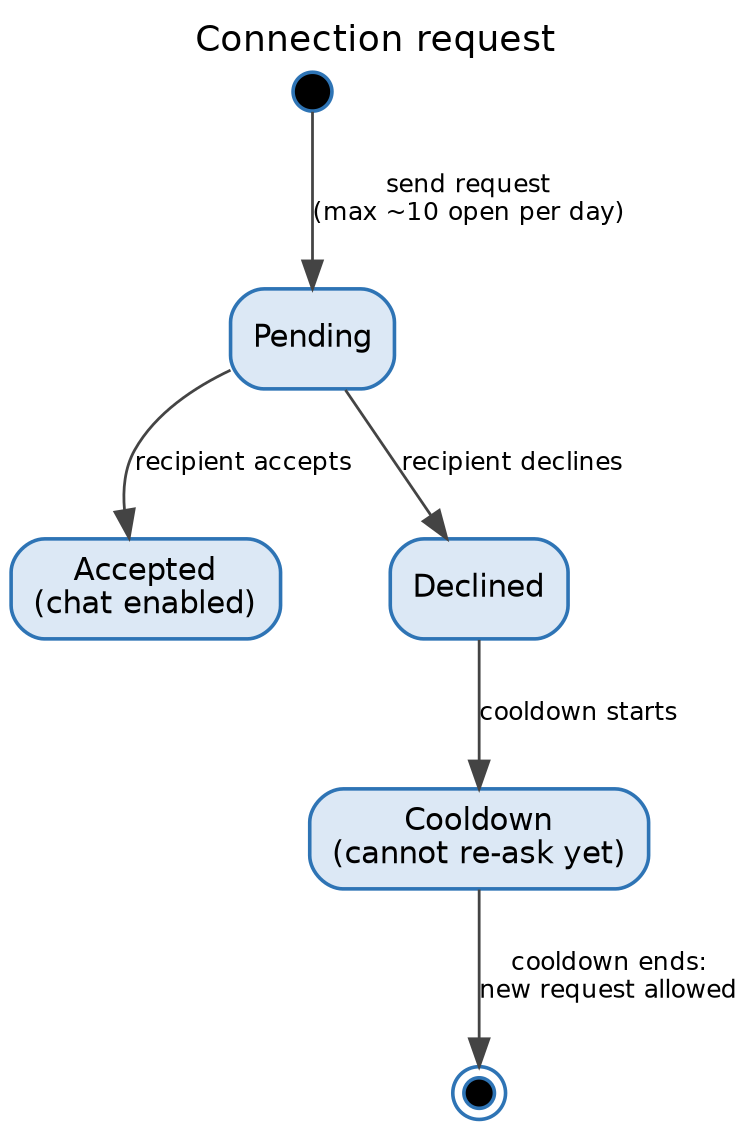
\includegraphics[width=0.48\linewidth]{figures/fig13a.png}\hfill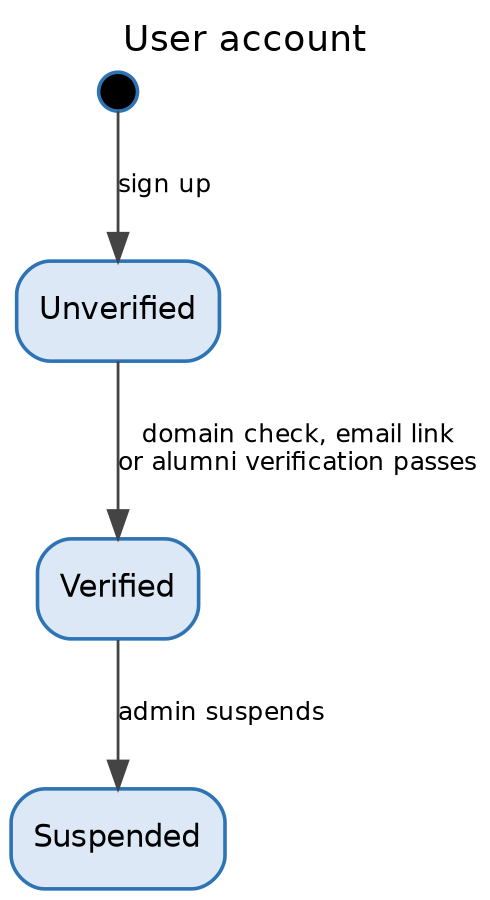
\includegraphics[width=0.48\linewidth]{figures/fig13b.png}
\caption{States of a connection request (left) and a user account (right)}\end{figure}
\begin{figure}[H]\centering
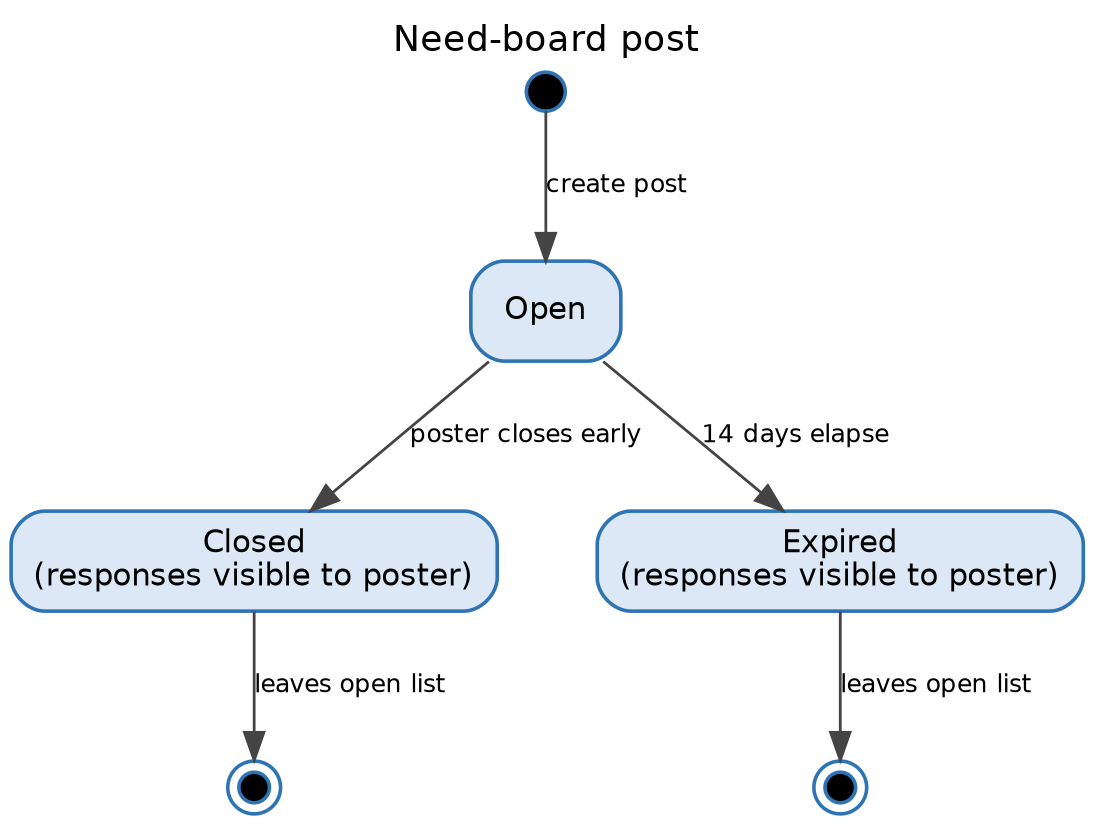
\includegraphics[width=0.48\linewidth]{figures/fig14a.png}\hfill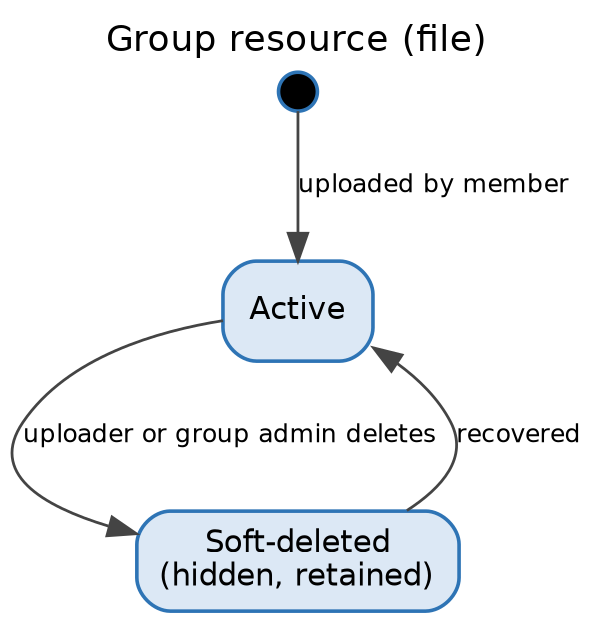
\includegraphics[width=0.48\linewidth]{figures/fig14b.png}
\caption{States of a need-board post (left) and a group file (right)}\end{figure}
\section{Use Case Summary}
Use case names match the labels in the use case diagrams (Figures 2 and 3).

{\small
\begin{longtable}{@{}l >{\raggedright\arraybackslash}p{50mm} >{\raggedright\arraybackslash}p{38mm} >{\raggedright\arraybackslash}p{24mm} >{\raggedright\arraybackslash}p{22mm}@{}}
\toprule
\textbf{ID} & \textbf{Use case} & \textbf{Primary actor(s)} & \textbf{User stories} & \textbf{SRS requirement}\\\midrule\endhead
\bottomrule\endfoot
UC1 & Sign in with Microsoft & Student; Microsoft Entra ID & US1.1 & FR1.1\\
UC2 & Verify IBA domain (server-side) & System; Microsoft Entra ID & US1.1 & FR1.1\\
UC3 & Sign up with email and password, verify & Student, Alumnus & US1.2, US1.3 & FR1.2\\
UC4 & Verify alumni status & Alumnus; University Administration & US1.4 & FR1.3\\
UC5 & Create / edit profile & Verified User & US1.5, US1.6, US1.7 & FR1.4\\
UC6 & Set available to advise & Senior & US1.8 & FR1.5\\
UC7 & Search and filter directory & Verified User & US2.2, US2.3, US2.4, US2.5 & FR2.2, FR2.3\\
UC8 & View member profile & Verified User & US2.1, US2.6 & FR2.1\\
UC9 & Send connection request & Verified User & US3.1, US3.2 & FR3.1\\
UC10 & Accept / decline request & Verified User & US3.3, US3.4 & FR3.2, FR3.3\\
UC11 & Chat with accepted connection & Verified User & US3.5, US3.6, US3.7 & FR3.4, FR3.5\\
UC12 & Post a need & Verified User & US4.1 & FR4.1\\
UC13 & Browse and respond to needs & Verified User & US4.2, US4.3 & FR4.2, FR4.3\\
UC14 & Close need post & Verified User (post author) & US4.4, US4.5 & FR4.4\\
UC15 & Create group & Verified User & US5.1, US5.4 & FR5.1, FR5.3\\
UC16 & Join group via invite link & Verified User & US5.3 & FR5.2\\
UC17 & Invite / add members & Group Admin & US5.2 & FR5.2\\
UC18 & Upload resource & Group Member & US6.1, US6.2 & FR6.1\\
UC19 & View / download resource & Group Member & US6.3 & FR6.2\\
UC20 & Delete resource (soft delete) & Group Member (uploader), Group Admin & US6.4 & FR6.3\\
UC21 & Create quiz (MCQ, true/false) & Group Member & US7.1 & FR7.1\\
UC22 & Attempt quiz & Group Member & US7.2 & FR7.2\\
UC23 & View personal score history & Group Member & US7.3 & FR7.3\\
UC24 & Report content & Verified User & US8.1 & FR8.1\\
UC25 & Review report queue & Moderator / Admin & US8.2 & FR8.2\\
UC26 & Hide / remove content & Moderator / Admin & US8.3 & FR8.2\\
UC27 & Warn user & Moderator / Admin & US8.3 & FR8.2\\
UC28 & Suspend account & Moderator / Admin & US8.3 & FR8.2\\
\end{longtable}}
\section{User Stories}
Each story follows the form ''As a [role], I want [goal], so that [benefit]''. Acceptance criteria are written as testable conditions. Priority is High or Medium, as in the SRS, and delivery follows the SRS build order: profiles and search, connections and chat, need board, groups and resources, then quizzes.

\subsection*{Epic E1: Identity and Verified Profile}
{\small
\begin{longtable}{@{}p{15mm} >{\raggedright\arraybackslash}p{45mm} >{\raggedright\arraybackslash}p{82mm} p{12mm}@{}}
\toprule
\textbf{ID / SRS} & \textbf{User story} & \textbf{Acceptance criteria} & \textbf{Priority}\\\midrule\endhead
\bottomrule\endfoot

US1.1\newline{\color{mid}FR1.1} & As a IBA student, I want to sign in with my IBA Microsoft account, so that I can join the network without managing another password. & \begin{minipage}[t]{\linewidth}\begin{itemize}[leftmargin=9pt,topsep=0pt,itemsep=1pt]\item Given I choose Microsoft sign-in, when I authenticate and my verified email is on the khi.iba.edu.pk domain, then I am signed in and an account is created if I am new.\item Given my email is not on the IBA domain or is not verified, when sign-in completes, then access is refused with a clear message and no account is created.\item Given I am signing in for the first time, then I am taken to profile setup.\end{itemize}\vspace{2pt}\end{minipage} & High\\\midrule
US1.2\newline{\color{mid}FR1.2} & As a person who cannot use a university account, I want to register with email and password and verify my email, so that I can still access the network. & \begin{minipage}[t]{\linewidth}\begin{itemize}[leftmargin=9pt,topsep=0pt,itemsep=1pt]\item Given I register with an email and password, then a verification email is sent and I cannot use the platform until I verify.\item Given I have verified my email, then I receive the same kind of profile as a Microsoft sign-in user.\item Given I set a password, then it is stored hashed (bcrypt), never in plain text.\end{itemize}\vspace{2pt}\end{minipage} & High\\\midrule
US1.3\newline{\color{mid}FR1.2} & As a registered user, I want to reset a forgotten password and change my password, so that I can recover and secure my account. & \begin{minipage}[t]{\linewidth}\begin{itemize}[leftmargin=9pt,topsep=0pt,itemsep=1pt]\item Given I request a reset with my registered email, then a reset email is sent.\item Given I am signed in, when I submit a new password, then it is saved and used for later sign-ins.\end{itemize}\vspace{2pt}\end{minipage} & High\\\midrule
US1.4\newline{\color{mid}FR1.3} & As a alumnus without an active IBA email, I want to verify with an administration code or invite, or with my personal email, so that I can join as an alumnus. & \begin{minipage}[t]{\linewidth}\begin{itemize}[leftmargin=9pt,topsep=0pt,itemsep=1pt]\item Given I enter a valid code or invite issued by the administration, then my account is verified as an alumnus.\item Given my personal email matches the university alumni list, then my account is verified as an alumnus.\item Given neither applies, then verification is refused and no alumnus access is given.\end{itemize}\vspace{2pt}\end{minipage} & High\\\midrule
US1.5\newline{\color{mid}FR1.4} & As a new user, I want to complete my profile with the required details, so that other members can find and understand who I am. & \begin{minipage}[t]{\linewidth}\begin{itemize}[leftmargin=9pt,topsep=0pt,itemsep=1pt]\item Given I am setting up a profile, then name, batch, programme and department, current semester, a short bio, and skills are required before I can finish.\item Courses taken, the available-to-advise flag, and an avatar are optional.\item Profile details are self-declared and are not shown as verified.\end{itemize}\vspace{2pt}\end{minipage} & High\\\midrule
US1.6\newline{\color{mid}FR1.4} & As a member, I want to edit my profile and avatar at any time, so that my information stays current. & \begin{minipage}[t]{\linewidth}\begin{itemize}[leftmargin=9pt,topsep=0pt,itemsep=1pt]\item Given I save changes, then they appear on my profile and in search results.\item Given I upload an avatar, then only image files are accepted and the file is stored in object storage.\end{itemize}\vspace{2pt}\end{minipage} & Medium\\\midrule
US1.7\newline{\color{mid}FR1.4} & As a alumnus, I want to add my field and company to my profile, so that students can find me by career area. & \begin{minipage}[t]{\linewidth}\begin{itemize}[leftmargin=9pt,topsep=0pt,itemsep=1pt]\item Given I am an alumnus, then my profile includes field and company.\item Given I save them, then they can be used as alumni search filters.\end{itemize}\vspace{2pt}\end{minipage} & Medium\\\midrule
US1.8\newline{\color{mid}FR1.5} & As a senior, I want to mark myself as available to advise and choose the specific courses I can help with, so that students looking for those courses can find me. & \begin{minipage}[t]{\linewidth}\begin{itemize}[leftmargin=9pt,topsep=0pt,itemsep=1pt]\item Given I turn the toggle on, then I can select the specific courses I can advise on.\item Given the toggle is on, then my profile and search results show an ''available to advise'' badge.\item Given I turn the toggle off, then the badge is removed and I no longer match the availability filter.\end{itemize}\vspace{2pt}\end{minipage} & High\\\midrule
\end{longtable}}
\subsection*{Epic E2: Directory and Search}
{\small
\begin{longtable}{@{}p{15mm} >{\raggedright\arraybackslash}p{45mm} >{\raggedright\arraybackslash}p{82mm} p{12mm}@{}}
\toprule
\textbf{ID / SRS} & \textbf{User story} & \textbf{Acceptance criteria} & \textbf{Priority}\\\midrule\endhead
\bottomrule\endfoot

US2.1\newline{\color{mid}FR2.1} & As a verified user, I want to browse a paginated directory of members, so that I can discover people on campus. & \begin{minipage}[t]{\linewidth}\begin{itemize}[leftmargin=9pt,topsep=0pt,itemsep=1pt]\item Given I am signed in, then I see a paginated list of verified members.\item Each result links to that member's profile.\item No email or other contact detail is shown in the directory, and the directory cannot be viewed without a verified sign-in.\end{itemize}\vspace{2pt}\end{minipage} & High\\\midrule
US2.2\newline{\color{mid}FR2.2} & As a verified user, I want to search by free text across name, skill and course, so that I can quickly find someone for my need. & \begin{minipage}[t]{\linewidth}\begin{itemize}[leftmargin=9pt,topsep=0pt,itemsep=1pt]\item Given I enter a keyword, then results include members whose name, skill or course matches.\item Search returns within 2 seconds at the 95th percentile.\end{itemize}\vspace{2pt}\end{minipage} & High\\\midrule
US2.3\newline{\color{mid}FR2.3} & As a verified user, I want to filter members by course, skill, availability to advise, batch, and department or programme, so that I can narrow results to the right people. & \begin{minipage}[t]{\linewidth}\begin{itemize}[leftmargin=9pt,topsep=0pt,itemsep=1pt]\item Given I select several filters, then results match all of them.\item Filters are offered in the priority order: course, skill, availability to advise, batch, department/programme.\item Given I clear the filters, then the full directory is shown again.\end{itemize}\vspace{2pt}\end{minipage} & High\\\midrule
US2.4\newline{\color{mid}FR2.3} & As a student registering for a course, I want to filter by course and availability to advise, so that I can find seniors who can guide me in that course. & \begin{minipage}[t]{\linewidth}\begin{itemize}[leftmargin=9pt,topsep=0pt,itemsep=1pt]\item Given I filter by a course and by availability to advise, then only members who listed that course and are available to advise are shown.\item Each such result shows the ''available to advise'' badge.\end{itemize}\vspace{2pt}\end{minipage} & High\\\midrule
US2.5\newline{\color{mid}FR2.3} & As a student, I want to filter alumni by field and company, so that I can find alumni working in a field I want to enter. & \begin{minipage}[t]{\linewidth}\begin{itemize}[leftmargin=9pt,topsep=0pt,itemsep=1pt]\item Given I view alumni results, then field and company filters are available.\item Given I apply them, then only matching alumni are shown.\end{itemize}\vspace{2pt}\end{minipage} & Medium\\\midrule
US2.6\newline{\color{mid}FR2.1} & As a verified user, I want to open a member's profile, so that I can decide whether to connect with them. & \begin{minipage}[t]{\linewidth}\begin{itemize}[leftmargin=9pt,topsep=0pt,itemsep=1pt]\item Given I open a profile, then I see name, batch, programme, department, bio, skills, courses, and the advise badge where applicable.\item Given we are not connected, then their email is not shown.\end{itemize}\vspace{2pt}\end{minipage} & High\\\midrule
\end{longtable}}
\subsection*{Epic E3: Connections and Messaging}
{\small
\begin{longtable}{@{}p{15mm} >{\raggedright\arraybackslash}p{45mm} >{\raggedright\arraybackslash}p{82mm} p{12mm}@{}}
\toprule
\textbf{ID / SRS} & \textbf{User story} & \textbf{Acceptance criteria} & \textbf{Priority}\\\midrule\endhead
\bottomrule\endfoot

US3.1\newline{\color{mid}FR3.1} & As a verified user, I want to send a connection request with a short context note, so that the person knows why I am reaching out. & \begin{minipage}[t]{\linewidth}\begin{itemize}[leftmargin=9pt,topsep=0pt,itemsep=1pt]\item Given I am on a profile, when I write a note and send, then a pending request is created and appears in my outgoing list.\item Given the request is sent, then the recipient is notified by email.\end{itemize}\vspace{2pt}\end{minipage} & High\\\midrule
US3.2\newline{\color{mid}FR3.1} & As a member, I want to have the number of requests limited and a cooldown applied, so that I am not spammed by repeated requests. & \begin{minipage}[t]{\linewidth}\begin{itemize}[leftmargin=9pt,topsep=0pt,itemsep=1pt]\item Given I already have about ten open requests today, when I try to send another, then it is blocked with an explanation.\item Given I asked the same person recently, when I try again during the cooldown, then it is blocked and I am told to wait.\end{itemize}\vspace{2pt}\end{minipage} & Medium\\\midrule
US3.3\newline{\color{mid}FR3.2} & As a request recipient, I want to accept or decline a request, so that I control who can message me. & \begin{minipage}[t]{\linewidth}\begin{itemize}[leftmargin=9pt,topsep=0pt,itemsep=1pt]\item Given I accept, then the connection is created and private chat is enabled for both people.\item Given I decline, then the requester sees the request as declined and chat stays disabled.\end{itemize}\vspace{2pt}\end{minipage} & High\\\midrule
US3.4\newline{\color{mid}FR3.3} & As a member, I want to see my requests in an inbox with incoming, outgoing and accepted views, so that I can keep track of my connections. & \begin{minipage}[t]{\linewidth}\begin{itemize}[leftmargin=9pt,topsep=0pt,itemsep=1pt]\item Given I open the inbox, then I can switch between incoming, outgoing and accepted requests.\item Each entry shows the person, context note and status.\end{itemize}\vspace{2pt}\end{minipage} & High\\\midrule
US3.5\newline{\color{mid}FR3.4} & As a connected member, I want to send private messages to my accepted connections, so that I can get help or coordinate directly. & \begin{minipage}[t]{\linewidth}\begin{itemize}[leftmargin=9pt,topsep=0pt,itemsep=1pt]\item Given a connection is accepted, then both people can send and read messages in a private thread.\item Given no accepted connection exists, then sending a message is refused.\item Messages are shown in order with their time.\end{itemize}\vspace{2pt}\end{minipage} & High\\\midrule
US3.6\newline{\color{mid}FR3.4} & As a member, I want to see unread indicators on my conversations, so that I do not miss new messages. & \begin{minipage}[t]{\linewidth}\begin{itemize}[leftmargin=9pt,topsep=0pt,itemsep=1pt]\item Given I have unread messages, then an unread indicator is shown.\item Given I open the thread, then the messages are marked as read.\end{itemize}\vspace{2pt}\end{minipage} & Medium\\\midrule
US3.7\newline{\color{mid}FR3.5} & As a member, I want to keep my email hidden until I accept a connection, so that my contact details stay private. & \begin{minipage}[t]{\linewidth}\begin{itemize}[leftmargin=9pt,topsep=0pt,itemsep=1pt]\item Given I am not connected with someone, then they cannot see my email anywhere.\item Given a connection is accepted, then each person can see the other's email.\end{itemize}\vspace{2pt}\end{minipage} & High\\\midrule
\end{longtable}}
\subsection*{Epic E4: Need Board}
{\small
\begin{longtable}{@{}p{15mm} >{\raggedright\arraybackslash}p{45mm} >{\raggedright\arraybackslash}p{82mm} p{12mm}@{}}
\toprule
\textbf{ID / SRS} & \textbf{User story} & \textbf{Acceptance criteria} & \textbf{Priority}\\\midrule\endhead
\bottomrule\endfoot

US4.1\newline{\color{mid}FR4.1} & As a verified user, I want to post a need with a type and optional course or department tag, so that the right people can find and respond to it. & \begin{minipage}[t]{\linewidth}\begin{itemize}[leftmargin=9pt,topsep=0pt,itemsep=1pt]\item Given I create a post, then I choose a type (study partner, project teammate, course advice, career advice), a title and a body, and may add a course or department tag.\item Given I publish, then the post is open and visible to all verified users.\end{itemize}\vspace{2pt}\end{minipage} & High\\\midrule
US4.2\newline{\color{mid}FR4.2} & As a verified user, I want to browse and filter the need board, so that I can find needs I can help with. & \begin{minipage}[t]{\linewidth}\begin{itemize}[leftmargin=9pt,topsep=0pt,itemsep=1pt]\item Given I open the board, then I see only open posts.\item Given I filter by type or by course/department tag, then the list is narrowed accordingly.\end{itemize}\vspace{2pt}\end{minipage} & High\\\midrule
US4.3\newline{\color{mid}FR4.3} & As a verified user, I want to respond to a post, so that I can offer help or join the person. & \begin{minipage}[t]{\linewidth}\begin{itemize}[leftmargin=9pt,topsep=0pt,itemsep=1pt]\item Given I respond, then a connection request opens pre-filled with the post context.\item The usual request limits and cooldown apply.\item The poster can see my response.\end{itemize}\vspace{2pt}\end{minipage} & High\\\midrule
US4.4\newline{\color{mid}FR4.4} & As a post author, I want to close my post once it is resolved, so that people stop responding to a finished need. & \begin{minipage}[t]{\linewidth}\begin{itemize}[leftmargin=9pt,topsep=0pt,itemsep=1pt]\item Given I close my post, then it leaves the open list.\item Responses to the post remain visible to me after closing.\end{itemize}\vspace{2pt}\end{minipage} & Medium\\\midrule
US4.5\newline{\color{mid}FR4.4} & As a post author, I want to have my post expire automatically after 14 days, so that the board does not fill with stale posts. & \begin{minipage}[t]{\linewidth}\begin{itemize}[leftmargin=9pt,topsep=0pt,itemsep=1pt]\item Given a post is 14 days old, then it expires and leaves the open list.\item Responses to an expired post remain visible to the author.\end{itemize}\vspace{2pt}\end{minipage} & High\\\midrule
\end{longtable}}
\subsection*{Epic E5: Study and Project Groups}
{\small
\begin{longtable}{@{}p{15mm} >{\raggedright\arraybackslash}p{45mm} >{\raggedright\arraybackslash}p{82mm} p{12mm}@{}}
\toprule
\textbf{ID / SRS} & \textbf{User story} & \textbf{Acceptance criteria} & \textbf{Priority}\\\midrule\endhead
\bottomrule\endfoot

US5.1\newline{\color{mid}FR5.1} & As a verified user, I want to create a study or project group, so that I can organise work with my peers. & \begin{minipage}[t]{\linewidth}\begin{itemize}[leftmargin=9pt,topsep=0pt,itemsep=1pt]\item Given I create a group, then I choose a name and a type label (study or project); the label changes no behaviour.\item I do not need to be connected to anyone or share a course to create a group.\item Given the group is created, then I become its group admin.\end{itemize}\vspace{2pt}\end{minipage} & High\\\midrule
US5.2\newline{\color{mid}FR5.2} & As a group creator, I want to add members by invite link or directly, so that I can bring in the right people. & \begin{minipage}[t]{\linewidth}\begin{itemize}[leftmargin=9pt,topsep=0pt,itemsep=1pt]\item Given I open my group, then I can generate an invite link.\item Given I choose a verified user, then I can add them directly.\end{itemize}\vspace{2pt}\end{minipage} & High\\\midrule
US5.3\newline{\color{mid}FR5.2} & As a verified user, I want to join a group using an invite link, so that I can access my group's material. & \begin{minipage}[t]{\linewidth}\begin{itemize}[leftmargin=9pt,topsep=0pt,itemsep=1pt]\item Given I open a valid invite link while signed in, then I become a member.\item Given the link is invalid, then I am refused entry.\end{itemize}\vspace{2pt}\end{minipage} & High\\\midrule
US5.4\newline{\color{mid}FR5.3} & As a group member, I want to have my group hidden from search and its content visible only to members, so that our material stays private. & \begin{minipage}[t]{\linewidth}\begin{itemize}[leftmargin=9pt,topsep=0pt,itemsep=1pt]\item Given a group exists, then it does not appear in the directory or any search.\item Given someone is not a member, then requests for the group's files or quizzes are denied.\end{itemize}\vspace{2pt}\end{minipage} & High\\\midrule
\end{longtable}}
\subsection*{Epic E6: Resource Sharing}
{\small
\begin{longtable}{@{}p{15mm} >{\raggedright\arraybackslash}p{45mm} >{\raggedright\arraybackslash}p{82mm} p{12mm}@{}}
\toprule
\textbf{ID / SRS} & \textbf{User story} & \textbf{Acceptance criteria} & \textbf{Priority}\\\midrule\endhead
\bottomrule\endfoot

US6.1\newline{\color{mid}FR6.1} & As a group member, I want to upload study material to my group, so that everyone in the group can use it. & \begin{minipage}[t]{\linewidth}\begin{itemize}[leftmargin=9pt,topsep=0pt,itemsep=1pt]\item Given I am a member, then I can upload PDF, DOCX, PPTX and image files of up to 25 MB each.\item Given the upload succeeds, then the file appears in the group list with the uploader and date.\end{itemize}\vspace{2pt}\end{minipage} & High\\\midrule
US6.2\newline{\color{mid}FR6.1} & As a group member, I want to be stopped from uploading unsupported or oversized files, so that the group stays safe and within limits. & \begin{minipage}[t]{\linewidth}\begin{itemize}[leftmargin=9pt,topsep=0pt,itemsep=1pt]\item Given I upload an archive or executable, then it is rejected with a clear message.\item Given a file is larger than 25 MB, then it is rejected with a clear message.\end{itemize}\vspace{2pt}\end{minipage} & High\\\midrule
US6.3\newline{\color{mid}FR6.2} & As a group member, I want to view and download files in my group, so that I can study from the shared material. & \begin{minipage}[t]{\linewidth}\begin{itemize}[leftmargin=9pt,topsep=0pt,itemsep=1pt]\item Given I am a member, then I can download any file that has not been deleted.\item Given I am not a member, then download is denied.\end{itemize}\vspace{2pt}\end{minipage} & High\\\midrule
US6.4\newline{\color{mid}FR6.3} & As a uploader or group admin, I want to delete a file, so that mistaken or outdated files can be removed. & \begin{minipage}[t]{\linewidth}\begin{itemize}[leftmargin=9pt,topsep=0pt,itemsep=1pt]\item Given I am the uploader or the group admin, then I can delete the file.\item Given I am another member, then deletion is not available to me.\item Given a file is deleted, then it is soft-deleted: hidden from members but retained for recovery or audit.\end{itemize}\vspace{2pt}\end{minipage} & Medium\\\midrule
\end{longtable}}
\subsection*{Epic E7: Practice Quizzes \vone{removed from scope}}
{\small
\begin{longtable}{@{}p{15mm} >{\raggedright\arraybackslash}p{45mm} >{\raggedright\arraybackslash}p{82mm} p{12mm}@{}}
\toprule
\textbf{ID / SRS} & \textbf{User story} & \textbf{Acceptance criteria} & \textbf{Priority}\\\midrule\endhead
\bottomrule\endfoot

US7.1\newline{\color{mid}FR7.1} & As a group member, I want to create a quiz by writing questions manually, so that my group can practise from our material. & \begin{minipage}[t]{\linewidth}\begin{itemize}[leftmargin=9pt,topsep=0pt,itemsep=1pt]\item Given I create a quiz, then I can add multiple-choice and true/false questions and mark the correct answers.\item Given I save, then the quiz appears in the group.\item Questions are entered by members; no AI generation is provided.\end{itemize}\vspace{2pt}\end{minipage} & High\\\midrule
US7.2\newline{\color{mid}FR7.2} & As a group member, I want to attempt a quiz and see my score, so that I can test my understanding. & \begin{minipage}[t]{\linewidth}\begin{itemize}[leftmargin=9pt,topsep=0pt,itemsep=1pt]\item Given I answer all questions and submit, then my score is shown.\item Given I submit, then the attempt is recorded with score and date.\end{itemize}\vspace{2pt}\end{minipage} & High\\\midrule
US7.3\newline{\color{mid}FR7.3} & As a group member, I want to see my past attempts and a chart of my scores over time, so that I can track my progress. & \begin{minipage}[t]{\linewidth}\begin{itemize}[leftmargin=9pt,topsep=0pt,itemsep=1pt]\item Given I open a quiz, then I see a list of my attempts with score and date.\item Given I have several attempts, then a simple chart of my scores over time is shown.\item Only my own scores are shown; there are no group leaderboards.\end{itemize}\vspace{2pt}\end{minipage} & Medium\\\midrule
\end{longtable}}
\subsection*{Epic E8: Moderation and Administration}
{\small
\begin{longtable}{@{}p{15mm} >{\raggedright\arraybackslash}p{45mm} >{\raggedright\arraybackslash}p{82mm} p{12mm}@{}}
\toprule
\textbf{ID / SRS} & \textbf{User story} & \textbf{Acceptance criteria} & \textbf{Priority}\\\midrule\endhead
\bottomrule\endfoot

US8.1\newline{\color{mid}FR8.1} & As a verified user, I want to flag a profile, message, post, file, quiz or group, so that harmful content can be reviewed. & \begin{minipage}[t]{\linewidth}\begin{itemize}[leftmargin=9pt,topsep=0pt,itemsep=1pt]\item Given I flag an item, then I must give a reason.\item Given I submit, then a report is added to the admin queue.\end{itemize}\vspace{2pt}\end{minipage} & Medium\\\midrule
US8.2\newline{\color{mid}FR8.2} & As a moderator, I want to review the queue of reports in a simple admin panel, so that I can decide what to do about each one. & \begin{minipage}[t]{\linewidth}\begin{itemize}[leftmargin=9pt,topsep=0pt,itemsep=1pt]\item Given I open the panel, then I see open reports with the target, reporter and reason.\item Reports are handled by the project team and the course administrator; nothing is moderated automatically.\end{itemize}\vspace{2pt}\end{minipage} & Medium\\\midrule
US8.3\newline{\color{mid}FR8.2} & As a moderator, I want to hide or remove content, warn a user, or suspend an account, so that the community stays safe. & \begin{minipage}[t]{\linewidth}\begin{itemize}[leftmargin=9pt,topsep=0pt,itemsep=1pt]\item Given I choose hide/remove, then the content is no longer visible to members.\item Given I choose warn or suspend, then the action is recorded on the report.\item Given an account is suspended, then that user can no longer use the platform.\end{itemize}\vspace{2pt}\end{minipage} & Medium\\\midrule
\end{longtable}}
\end{document}
